%&LaTeX
\documentclass[11pt,a4paper]{article}
\usepackage[frenchb,english]{babel}
\usepackage[applemac]{inputenc}
\usepackage[OT1]{fontenc}
\usepackage[]{graphicx}
\usepackage{amsmath}
\usepackage{amsfonts}
\usepackage{amsthm}
\usepackage{amssymb}
\usepackage{mathrsfs}
\usepackage{tikz}
\graphicspath{ {./figures/} }
%\input{8bitdefs}

% marges
\topmargin 10pt
\headsep 10pt
\headheight 10pt
\marginparwidth 30pt
\oddsidemargin 40pt
\evensidemargin 40pt
\footskip 30pt
\textheight 670pt
\textwidth 420pt

\def\imp{\Rightarrow}
\def\gcro{\mbox{[\hspace{-.15em}[}}% intervalles d'entiers 
\def\dcro{\mbox{]\hspace{-.15em}]}}

\newcommand{\be} {\begin{enumerate}}
\newcommand{\ee} {\end{enumerate}}
\newcommand{\deb}{\begin{eqnarray*}}
\newcommand{\fin}{\end{eqnarray*}}
\newcommand{\ssi} {si et seulement si }
\newcommand{\D}{\mathrm{d}}
\newcommand{\Q}{\mathbb{Q}}
\newcommand{\Z}{\mathbb{Z}}
\newcommand{\N}{\mathbb{N}}
\newcommand{\R}{\mathbb{R}}
\newcommand{\C}{\mathbb{C}}
\newcommand{\F}{\mathbb{F}}
\newcommand{\U}{\mathbb{U}}
\newcommand{\re}{\,\mathrm{Re}\,}
\newcommand{\im}{\,\mathrm{Im}\,}
\newcommand{\ord}{\mathrm{ord}}
\newcommand{\Gal}{\mathrm{Gal}}
\newcommand{\legendre}[2]{\genfrac{(}{)}{}{}{#1}{#2}}


\title{Solutions to David A.Cox  "Galois Theory''}

\refstepcounter{section} \refstepcounter{section}
\refstepcounter{section} \refstepcounter{section}
\refstepcounter{section}\refstepcounter{section}\refstepcounter{section}\refstepcounter{section}
\refstepcounter{section}\refstepcounter{section}\refstepcounter{section}\refstepcounter{section}
\refstepcounter{section}\refstepcounter{section}


\begin{document}



\section{Chapter 15 : THE LEMNISCATE}

\subsection{DIVISION POINTS AND ARC LENGTH}

\paragraph{Ex. 15.1.1}{\it Prove that the numbers described in Abel's theorem at the beginning of the chapter are precisely those in Theorem 10.2.1, provided we replace ``product of several numbers'' with ``product of distinct numbers'' in Abel's statement of the theorem.
}
\begin{proof}
The numbers described in Theorem 10.2.1 are the integers $n = 2^s p_1\cdots p_r$, where $p_1,\ldots,p_r$ are distinct Fermat primes, of the form $p_k = 2^{n_k} + 1$. Thus these numbers are the product of {\it distinct} numbers of the form $2^m$, or $2^{m}+1$, where $2^{m} + 1$ is prime, as described in the Theorem of Abel.
\end{proof}

\paragraph{Ex. 15.1.2}{\it Show that in polar coordinates, the equation of the lemniscate is $r^2 = \cos(2\theta)$.
}
\begin{proof}
By definition, a point $M = (x,y) \in \R^2$ is a point of the lemniscate $L$ if and only if
$$(x^2 + y^2)^2 = x^2 - y^2.$$ 
If $(r,\theta)$ are polar coordinates of $M = M(r,\theta)$, then $x = r \cos\theta, y = r \sin\theta$, thus, using $\cos^2 \theta + \sin^2 \theta = 1$, and $\cos(2\theta) = \cos^2 \theta) - \sin^2 \theta$, we obtain
\begin{align*}
M(r,\theta) \in L & \iff (r^2 \cos^2\theta + r^2 \sin^2\theta)^2 = r^2 \cos^2\theta - r^2 \sin^2\theta\\
&\iff r^4 = r^2 \cos(2\theta)\\
&\iff r^2 = \cos(2\theta).
\end{align*}
The equation of the lemniscate is $r^2 = \cos(2\theta)$.
\end{proof}


\paragraph{Ex. 15.1.3}{\it Prove that the two improper integrals $\int_0^1 (1-t^4)^{-1/2} \mathrm{d}t$ and $\int_{-1}^0 (1-t^4)^{-1/2} \mathrm{d}t$ converge.
}
\begin{proof}
 The map $t \mapsto (1-t^4)^{-1/2}$ is continuous on $[0,1[$, thus $t \mapsto(1-t^4)^{-1/2} \mathrm{d}t$ is summable on $[1,x]$ for all $x \in [0,1]$.  

Since $1-t^4 = (1-t)(1+t+t^2+t^3)$, $(1-t^4)^{-1/2} \sim [4(1-t)]^{-1/2}$ in the neighborhood of $1$. The Riemann Criterium shows that $\int_0^1 (1-t)^{-\alpha} \mathrm{d}t$ converges if  $\alpha  < 1$, and here $\alpha = 1/2$. Since $(1-t^4)^{-1/2} >0$, this is sufficient to prove that $\int_0^1 (1-t^4)^{-1/2} \mathrm{d}t$ converges.

Since $t \mapsto (1-t^4)^{-1/2}$ is even, the same is true in the neighborhood of $-1$, thus $\int_{-1}^0 (1-t^4)^{-1/2} \mathrm{d}t$ converges.
\end{proof}

\paragraph{Ex. 15.1.4}{\it  Prove the arc length formula stated in (15.6)}
\begin{proof}
 Here the equation of the ellipse $E$ is
 $$x^2 + \frac{y^2}{b^2} = 1,$$
 with eccentricity $k = \sqrt{1- b^2}$.

We compute the arc length $l$ of (E) between $x = u, y=v\ (-1<u<v<1)$ on the upper part of the curve. Then
$$l =  \int_u^v \sqrt{1+\left( \frac{\D y}{\D x}\right)^2}\  \D x,$$
where $y = f(x) = b \sqrt{1-x^2}.$ Then $f'(x) =  \frac{\D y}{\D x }= -\frac{2x}{\sqrt{1-x^2}}$, thus
\begin{align*}
l &=  \int_u^v \sqrt{1+\left(\frac{bx}{\sqrt{1-x^2}}\right)^2}\  \D x\\
&=\int_u^v \sqrt{\frac{1 - x^2 + b^2 x^2}{1-x^2}}\  \D x\\
&=\int_u^v \sqrt{\frac{1 - k^2 x^2}{1-x^2}}\  \D x\\
\end{align*}
We have proved
$$l =  \int_u^v \sqrt{1+\left( \frac{\D y}{\D x}\right)^2}\  \D x = \int_u^v \sqrt{\frac{1 - k^2 x^2}{1-x^2}}\  \D x = \int_u^v \frac{\sqrt{(1-x^2)(1 - k^2 x^2)}}{1-x^2}\  \D x.$$
The arc length of the ellipse is given by an elliptic integral.
\end{proof}

\paragraph{Ex. 15.1.5}{\it  Shows that (15.7) reduces to $(x^2+y^2)^2 = x^2 -y^2$ when $a=b = 1/\sqrt{2}$.
}
\begin{proof}
 If we take $a=b=1/\sqrt{2}$ in the formula of the ovals of Cassini
 $$((x-a)^2 + y^2)((x+a)^2 + y^2) = b^4,$$
 we obtain
 \begin{align*}
 \frac{1}{4} &= \left[ \left(x - \frac{1}{\sqrt{2}} \right)^2 + y^2\right ] \left[ \left(x + \frac{1}{\sqrt{2}} \right)^2 + y^2\right ]  \\
 &=\left( x^2+y^2 +\frac{1}{2}  - \sqrt{2}\, x \right)\left( x^2+y^2 +\frac{1}{2}  + \sqrt{2}\, x \right)\\
 &=\left((x^2 + y^2 + \frac{1}{2}\right)^2 - 2 x^2\\
 &=(x^2+y^2)^2  + (x^2+y^2) - 2 x^2\\
 &= (x^2+y^2)^2 + y^2 -x^2 + \frac{1}{4}.
 \end{align*}
 Therefore, for $a=b =1/\sqrt{2}$, the equation $((x-a)^2 + y^2)((x+a)^2 + y^2) = b^4$ reduces to
 $$(x^2 + y^2)^2 = x^2 - y^2,$$
 which is the equation of the Lemniscate.
\end{proof}


\paragraph{Ex. 15.1.6}{\it Let $n>0$ be an odd integer, and assume that the $n$-division points of the lemniscate can be constructed with straightedge and compass. Prove that the same is true for the $2n$-division points. Your proof should include a picture.
}

\begin{proof} Suppose that $n = 2N+1$ is odd, and consider $M_0=0, \ldots,M_{n-1}$  the $n$-divisions points, where $M_k$ has positive arc length $s_k = k \frac{2\varpi}{n},\ k=0,\ldots,n-1$.

Then $s_k = (2k) \frac{2\varpi}{2n}$, so that $N_{2k} = M_k$ is also a $2n$-division point. The other $2n$-division points are the points $N_{2k+1}$ corresponding to the arc length $k \frac{2\varpi}{n} + \frac{\varpi}{n} = (2k+1) \frac{\varpi}{n}$. Then the symmetric point $N'_{2k+1}$ about the $x$-axis has arc length 
$$\varpi - (2k+1) \frac{\varpi}{n} = \varpi - (2k+1) \frac{\varpi}{2N+1} = (N-k) \frac{2 \varpi}{n},$$
thus is the $n$-division point $M_{2n+1-k}$. This proves that the symmetric points $M'_0 = 0,\ldots,M'_{n-1}$  of $M_0,\ldots,M_{n-1}$ about the $x$-axis are $2n$-divisions points.


Therefore we can complete $M_0, M_1, \ldots,M_{n-1}$ by the symmetric points $M'_0 = O,\ldots,M'_{n-1}$ relative to the $x$-axis to obtain the $2n$-division points (the point $O$ is counted twice).

Since the $M_k$ can be constructed with straightedge and compass, the symmetric points $M'_k$ are also constructible, thus the $2n$-division points are constructible. 

Figure for $n=5$: the $10$-division points are $0,M'_2,M_1,M'_1,M_2,0,M_3,M'_3,M_4,M'_3$.
\begin{figure}[htbp]
\begin{center}
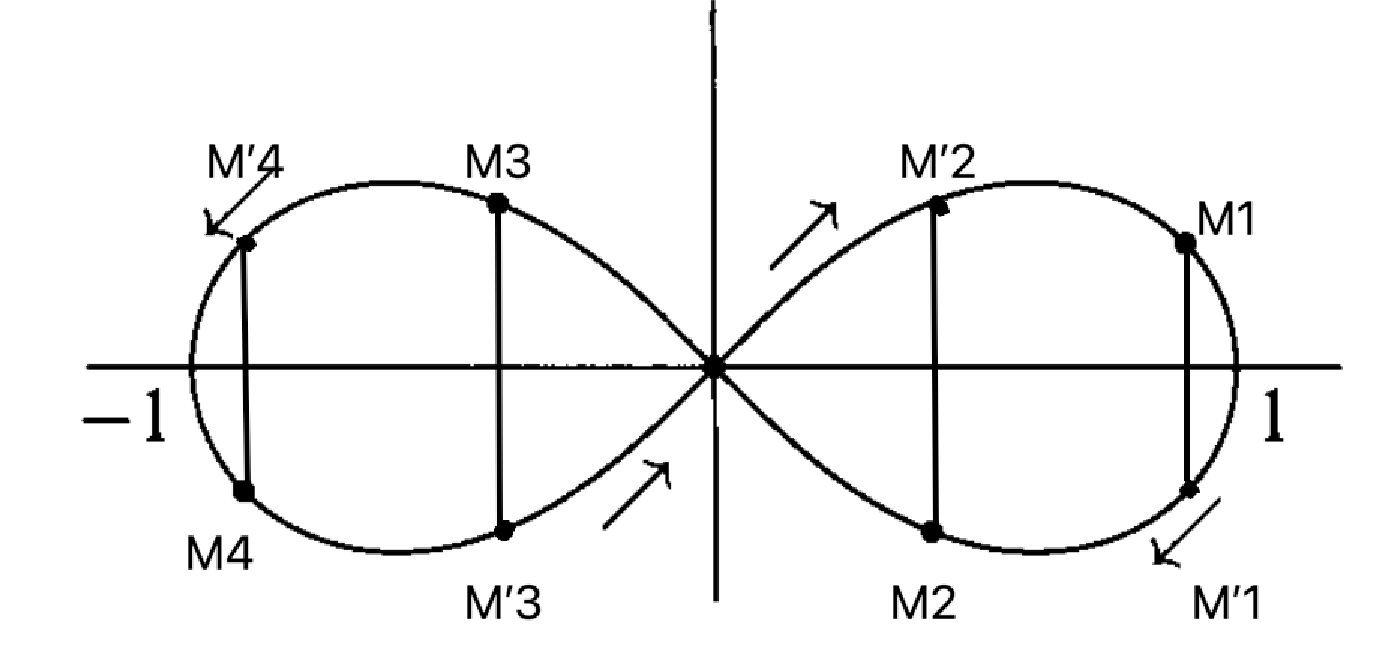
\includegraphics [width=8cm,height=4cm] {lemniscate.png}
\end{center}
\end{figure}
\end{proof}

\paragraph{Ex. 15.1.7}{\it Recall that in Greek geometry, the ellipse is defined to be the locus of all points whose {\bf sum} of distances to two given points is constant. Suppose instead we consider the locus of all points whose {\bf product} of distances to two given points is constant. Show that this leads to (15.7) when the given points are $(a,0),(-a,0)$ and the constant is $b^4$(*).
}

(*) Read $b^2$.

\begin{proof}
Let $\Gamma$ the locus of all points whose product of distances to two points $(a,0),(-a,0)$ is the constant $b^2$. Then
\begin{align*}
M(x,y) \in \Gamma & \iff \sqrt{(x-a)^2 + y^2}   \sqrt{(x+a)^2 + y^2}  = b^2\\
&\iff ((x-a)^2 + y^2)((x-a)^2 + y^2) = b^4.
\end{align*}
We obtain the formula of the ovals of Cassini.
\end{proof}


\subsection{THE LEMNISCATIC FUNCTION}
\paragraph{Ex. 15.2.1}{\it Give a careful proof of (15.9) using the hints given in the text.
}

\begin{proof}
By section 15.2, we know that $\varphi$ is $2\varpi$ periodic,
$$\varphi(s + 2\varpi) = \varphi(s),\qquad (s \in \R).$$
Moreover, for $-1 \leq r \leq 1$, and $\frac{-\varpi}{2} \leq s \leq \frac{\varpi}{2}$,
$$r = \varphi(s) \iff s = \int_0^r \frac{1}{\sqrt{1-t^4}} \D t.$$

Write $r' = \varphi(-s)\in [-1,1]$. Then for every $s \in [-\frac{\varpi}{2} ,\frac{\varpi}{2} ]$,
\begin{align*}
r' = \varphi(-s) & \iff -s = \int_0^{r'} \frac{1}{\sqrt{1-t^4}} \D t\\
&\iff -s = -\int _0^{-r'} \frac{1}{\sqrt{1-\tau^4}} \D \tau\qquad (\tau = -t)\\
&\iff s = \int _0^{-r'} \frac{1}{\sqrt{1-\tau^4}} \D \tau\\
&\iff -r' = \varphi(s)
\end{align*}
This proves that
\begin{align}
\varphi(-s) = - \varphi(s) \qquad \left (-\frac{\varpi}{2} \leq s \leq \frac{\varpi}{2} \right).
\end{align}

Write $M(s)$ the point on the lemniscate with signed arc length $s$. Consider $M' = M(s')$ the symmetric point of $M(s)$ about the origin. Since the lemniscate is symmetric about the origin, 
Consider first the case where $0 \leq s \leq \varpi$, then the signed arc length is the positive arc length. Let $M(s)$ the point on the lemniscate with arc length $s$. Then the symmetric point $M(s')$ about the $x$-axis is such that $r' = OM(s') = OM(s) = r$, thus, by definition of $\varphi$, $\varphi(s) = \varphi(s')$. The total arc length from $O = M(0)$ to $O = M(\varpi)$ in the first loop is $\varpi$, and the symmetry of the lemniscate about the $x$-axis implies that the arc length $\varpi - s$ between $M(s)$ and $O = M(\varpi)$ is equal to the arc length $s'$ between $O = M(0)$ and $M(s')$, thus
$s' = \varpi - s$. This proves
\begin{align}
\varphi(\varpi -s) = \varphi(s)\qquad (0 \leq s \leq \varpi).
\end{align} 

Now, if $\frac{\varpi}{2} \leq s \leq \varpi$, then $0\leq \varpi-s \leq \frac{\varpi}{2}$, thus, using (1), (2), (3)
$$
\left\{
\begin{array}{ll}
\varphi(s) &= \varphi(\varpi - s) = -\varphi(s- \varpi) = -\varphi(s + \varpi),\\
\varphi(-s) &= \varphi(\varpi- (-s)) =\varphi(s + \varpi).
\end{array}
\right.
$$
Therefore $\varphi(-s) = - \varphi(s)$ if $\frac{\varpi}{2} \leq s \leq \varpi$. Now, if we suppose $-\varpi \leq s \leq -\frac{\varpi}{2}$, then $\frac{\varpi}{2} \leq -s \leq \varpi$, so we can apply the last equality to $-s$: $\varphi(s) = \varphi(-(-s))= - \varphi(-s)$. This proves
\begin{align}
\varphi(-s) = \varphi(s) \qquad (-\varpi \leq s \leq \varpi).
\end{align}
Using the periodicity, if $s \in \R$, the is some $n \in \Z$ and $s' \in [-\varpi,\varpi[$ such that $s = 2n\varpi + s'$. Then 
$$\varphi(-s) = \varphi(-s - 2n\varpi) = \varphi(-s') = - \varphi(s') = -\varphi(s-2n\varphi) = - \varphi(s).$$
 We have proved
$$\varphi(-s) = \varphi(s) \qquad (s \in \R).$$
We can now complete (2) to $-\varpi \leq s \leq 0$. Then $0 \leq -s \leq \varpi$, and by (2) applied to $-s$, $\varphi(s + \varpi) = \varphi(-s) = -\varphi(s)$, thus
$$\varphi(\varpi -s) =  - \varphi(s - \varpi) = - \varphi(s+ \varpi) = \varphi(s)$$.

We have proved, for all $s \in \R$,
\begin{align*}
&\varphi(-s) = -\varphi(s)\\
&\varphi(\varpi - s) = \varphi(s).
\end{align*}
\end{proof}

\paragraph{Ex. 15.2.2}{\it Supply the details needed to complete the proof of Proposition 15.2.1.
}

\begin{proof}
The proof of Proposition 15.2.1 shows that
$$\varphi'(s)  = \sqrt{1 - \varphi^4(s)},\qquad 0 \leq s \leq \frac{\varpi}{2}.$$
By Exercise 3, parts (a) and (b), $\varphi'$ is even and has period $2 \varpi$, and by part (c),
$$\varphi'(\varpi - s) = - \varphi'(s), \qquad s \in \R.$$

Therefore, if $-\frac{\varpi}{2} \leq s \leq 0$, then
$$\varphi'(s) = - \varphi'(-s) =  -\sqrt{1 - \varphi^4(-s)} = - \sqrt{1 - \varphi^4(s)}.$$
Now, if $\frac{\varpi}{2} \leq s \leq \varpi$, then $0 \leq \varpi -s \leq \frac{\varpi}{2}$, thus 
$$\varphi'(s) = -\varphi'(\varpi - s) = -\sqrt{1 - \varphi^4(\varpi - s)} = - \sqrt{1 - \varphi^4(s)}.$$
If $-\varpi \leq s \leq -\frac{\varpi}{2}$, then $\frac{\varpi}{2} \leq -s  \leq \varpi$. Using the above equality, we obtain
$$\varphi'(s) = - \varphi(-s) = -  \sqrt{1 - \varphi^4(-s)} = - \sqrt{1 - \varphi^4(s)}.$$
We have proved
$$\varphi'^2(s) = 1 - \varphi^4(s), \qquad -\varpi \leq s \leq \varpi. $$
Now if $s$ is any real number, there is some $n\in \Z$ and $s' \in [-\varpi, \varpi[$ such that $s = 2n \varpi + s'$. Since $2\varpi$ is a period of $\varphi$ and $\varphi'$,
$$\varphi'^2(s) = \varphi'^2(s') = 1 -\varphi^4(s') = 1 - \varphi^4(s).$$
This complete the proof of Proposition 15.2.1.
\end{proof}

\paragraph{Ex. 15.2.3}{\it Here are some useful properties of $\varphi'$.
\be
\item[(a)] $\varphi$ has period $2\varpi$. Explain why this implies that the same is true for $\varphi'$.
\item[(b)] $\varphi$ is an odd function by (15.9). Explain why this implies that $\varphi'$ is even.
\item[(c)] Use (15.9) to prove that $\varphi'(\varpi -s) =  - \varphi'(s)$.
\item[(d)] Use Proposition 15.2.1 to prove that $\varphi''(s) = -2 \varphi^3(s)$.
\ee
}

\begin{proof}
\item[(a)] For all $s \in \R$, $\varphi(s +2 \varpi) = \varphi(s)$. By differentiation, and the chain rule,  we obtain
$$\varphi'(s + 2 \varphi)(s)= \varphi(s).$$
$\varphi'$ has period $2 \varpi$.
\item[(b)] Since $\varphi(-s) = - \varphi(s)$ for all $s \in \R$, the chain rule gives
$$- \varphi'(-s) = - \varphi'(s),$$
thus $\varphi'$ is even.
\item[(c)] By (15.9), $\varphi(\varpi - s) = \varphi(s)$ for all $s \in \R$. Then the chain rule gives $-\varphi'(\varpi -s) = \varphi'(s)$, thus
$$\varphi'(\varpi -s) = -\varphi'(s),\qquad s \in \R.$$
\item[(d)] By differentiation of $\varphi'^2(s) = 1 - \varphi^4(s)\ (s \in \R)$, we obtain
$$2 \varphi'(s) \varphi''(s) = -4 \varphi^3(s) \varphi'(s).$$
If $s \ne \frac{\varpi}{2} + n \varpi, n \in \Z$, then $\varphi'(s) \ne 0$, so that
$$\varphi''(s) = -2 \varphi^3(s),\qquad s \ne \frac{\varpi}{2} + n \varpi, n \in \Z.$$
If $s=\frac{\varpi}{2} + n \varpi $ for some integer $n \in \Z$, since $\varphi$ is infinitely differentiable, $\varphi''$ is continuous, therefore
$$\varphi''(s) = \lim_{t \to s, t\ne s} \varphi''(t) = \lim_{t \to s, t \ne s} (-2 \varphi^3(t)) = -2 \varphi^3(s).$$
Therefore
$$\varphi''(s) = -2 \varphi^3(s),\qquad s \in \R.$$
\end{proof}

\paragraph{Ex. 15.2.4}{\it Suppose that we define $\sin(x)$ by $y = \sin(x) \iff x = \int_0^y(1-t^2)^{-1/2} \D t$. Then define $\cos (x)$ to be $sin'(x)$. Use the method of Proposition 15.2.1 to prove the standard trigonometric identity $\cos^2(x) = 1 - \sin^2(x)$.
}

\begin{proof}
We obtain the analog of (15.9) as in Exercise 1: for all $x \in \R$,
\begin{align*}
\sin(-x) = - \sin(x),\\
\sin(\pi-x) = \sin(x).
\end{align*}

Now we use the definition of $\sin$: for all $y\in [-1,1]$, for all $x \in [-\frac{\pi}{2}, \frac{\pi}{2}]$,
$$y = \sin(x) \iff x = \int_0^y(1-t^2)^{-1/2} \D t,$$
where $\int_0^1(1-t^2)^{-1/2} \D t$ and $ \int_0^{-1}(1-t^2)^{-1/2} \D t$ converge.

If $x \in [0 , \frac{\pi}{2}[$, differentiating each side of
$$s = \int_0^{\sin(x)} \frac{1}{\sqrt{1-t^2}} \D t,$$
we obtain
$$1 = \frac{1}{\sqrt{1 - \sin^2(x)}} \sin'(x).$$
If $x = \frac{\pi}{2}$, then $\sin(x) = 1, \sin'(x) = 0$, thus $\sin'^2(x) = 1 - \sin^2(x)$.
Therefore
$$\cos(x) = \sin'(x) = \sqrt{1 - \sin^2(x)},\qquad 0 \leq x \leq \frac{\pi}{2}.$$
We extend the equality $\sin^2(x) + \cos^2(x) = 1$ to all $x \in \R$ as in Exercise 2.
\end{proof}

\paragraph{Ex. 15.2.5}{\it Here is Abel's proof of the addition law for $\varphi$.
\be
\item[(a)]
Let $g(x,y)$ be differentiable on $\R^2$, and set $h(u,v) = g\left(\frac{1}{2}(u+v), \frac{1}{2}(u-v)\right)$. Use the chain Rule to prove that
$$\frac{\partial h}{\partial v}(u,v) = \frac{1}{2}\frac{\partial g}{\partial x}\left(\frac{1}{2}(u+v), \frac{1}{2}(u-v)\right)-\frac{1}{2}\frac{\partial g}{\partial y}\left(\frac{1}{2}(u+v), \frac{1}{2}(u-v).\right)$$
\item[(b)] Use part (a) to show that $g(x,y) = g(x+y, 0)$ on, $\R^2$ if and only if $\frac{\partial g}{\partial x} = \frac{\partial g}{\partial y}$ on $\R^2$.
\item[(c)] Prove the addition law for $\varphi$ by applying part (b) to
$$g(x,y) = \frac{\varphi(x) \varphi'(y) + \varphi(y) \varphi'(x)}{1 + \varphi^2(x) \varphi^2(y)}.$$
Part (d) of Exercise 3 will be useful.
\ee
}

\begin{proof} 
\item[(a)] To apply the Chain Rule, we suppose that $g$ is continuously differentiable ($g \in C_1(\R^2)$). Write $x,y : \R^2 \to \R^2$ the two maps defined by
$$x(u,v) = \frac{1}{2}(u+v),\qquad y(u,v) = \frac{1}{2}(u-v),$$
Then 
$$\frac{\partial x}{\partial v}(u,v) = \frac{1}{2},\qquad \frac{\partial y}{\partial v}(u,v) = -\frac{1}{2},$$
and
$$h(u,v) = g(x(u,v),y(u,v)),\qquad (u,v)\in \R^2.$$
The Chain Rule gives
\begin{align*}
\frac{\partial h}{\partial v}(u,v)&=\frac{\partial g}{\partial x}\left(x(u,v),y(u,v)\right)\frac{\partial x}{\partial v}(u,v)+\frac{\partial g}{\partial y}\left(x(u,v),y(u,v)\right)\frac{\partial y}{\partial v}(u,v)\\
&=\frac{1}{2}\frac{\partial g}{\partial x}\left(\frac{1}{2}(u+v), \frac{1}{2}(u-v)\right)-\frac{1}{2}\frac{\partial g}{\partial y}\left(\frac{1}{2}(u+v), \frac{1}{2}(u-v)\right)
\end{align*}

\item[(b)] 

Suppose that $g(x+y,0) = g(x,y)$ for all $x,y \in \R$. Write $f(x) = g(x,0)$. Then $f$ is continuously differentiable, and $g(x,y) = f(x+y)$. By the Chain Rule, for all $(x,y) \in \R^2$,
$$
\frac{\partial g}{\partial x}(x,y) = f'(x+y) = \frac{\partial g}{\partial y}(x,y),
$$
therefore $\frac{\partial g}{\partial x} = \frac{\partial g}{\partial y}$ on $\R^2$.

\qquad

Conversely, suppose that $\frac{\partial g}{\partial x} = \frac{\partial g}{\partial y}$ on $\R^2$. Then, for all $(u,v) \in \R^2$,
$$\frac{\partial h}{\partial v}(u,v) = \frac{1}{2}\frac{\partial g}{\partial x}\left(\frac{1}{2}(u+v), \frac{1}{2}(u-v)\right)-\frac{1}{2}\frac{\partial g}{\partial y}\left(\frac{1}{2}(u+v), \frac{1}{2}(u-v) \right)= 0.$$
This means that for every fixed $u_0 \in \R$, the map $v \mapsto h(u_0,v)$ has a null derivative, thus is constant: $h(u_0,v) = h(u_0,0)$ for all $v \in \R$. Since this is true for every $u_0$, we obtain 
$$h(u,v) = h(u,0),\qquad \text{for all } u,v \in \R.$$
Write $f(u) = h(u,0)$ for all $u\in \R$. Then $f$ is continuously differentiable, and for all $u,v \in \R$, $h(u,v) = f(u)$ depends only of $u$.

By definition of $h$, this means that, for all $u,v \in \R$,
$$g\left(\frac{1}{2}(u+v), \frac{1}{2}(u-v)\right) = f(u).$$
Taking $v = u$ in $g\left(\frac{1}{2}(u+v), \frac{1}{2}(u-v)\right) = h(u,v) = h(u,0)$, we obtain $g(u,0) = h(u,u) = h(u,0)$, therefore
$$g(u,0) = h(u,u) = h(u,0) = h(u,v) = g\left(\frac{1}{2}(u+v), \frac{1}{2}(u-v)\right),$$
thus
$$g(u,0) = g\left(\frac{1}{2}(u+v), \frac{1}{2}(u-v)\right),\qquad u,v \in \R.$$
If $(x,y)$ is any pair in $\R^2$, there exists a unique pair $(u,v) \in \R^2$ such that $x = \frac{1}{2}(u+v), y = \frac{1}{2}(u-v)$, given by $u = x + y, v = x-y$. Therefore, the preceding equality implies that 
$$g(x+y,0) = g(x,y) ,\qquad x,y \in \R.$$ 

\item[(c)] Define $g : \R^2 \to \R$ by
$$g(x,y) = \frac{\varphi(x) \varphi'(y) + \varphi(y) \varphi'(x)}{1 + \varphi^2(x) \varphi^2(y)}.$$
The partial derivative of this quotient relative to the variable $x$ gives, using $\varphi''(x) = -2 \varphi^3(x)$ (see Exercise 3, part (d)), and $\varphi'(x)^2 = 1 -\varphi^4(x)$
\begin{align*}
&\left(1 + \varphi^2(x)\varphi^2(y)\right)^2 \frac{\partial g}{\partial x} (x,y) \\
&= \left(\varphi'(x) \varphi'(y) + \varphi(y) \varphi''(x)\right)\left(1+ \varphi^2(x)\varphi^2(y)\right) - 2 \varphi(x) \varphi'(x) \varphi^2(y) \left(\varphi(x) \varphi'(y)+ \varphi(y)\varphi'(x)\right)\\
&= \left(\varphi'(x) \varphi'(y) -2 \varphi(y)\varphi^3(x)\right)\left(1+ \varphi^2(x)\varphi^2(y)\right) - 2 \varphi(x) \varphi'(x) \varphi^2(y) \left(\varphi(x) \varphi'(y)+ \varphi(y)\varphi'(x)\right)\\
&=\varphi'(x) \varphi'(y) + \varphi'(x) \varphi'(y) \varphi^2(x) \varphi^2(y) - 2 \varphi(y) \varphi^3(x) - 2 \varphi^3(y)\varphi^5(x)\\
&  \qquad - 2 \varphi^2(x) \varphi^2(y) \varphi'(x)\varphi'(y) - 2 \varphi(x) \varphi^3(y) \varphi'(x)^2\\
&=\varphi'(x) \varphi'(y) + \varphi'(x) \varphi'(y) \varphi^2(x) \varphi^2(y) - 2 \varphi(y) \varphi^3(x) - 2 \varphi^3(y)\varphi^5(x)\\
&  \qquad - 2 \varphi^2(x) \varphi^2(y) \varphi'(x)\varphi'(y) - 2 \varphi(x) \varphi^3(y) (1 - \varphi^4(x))\\
&=\varphi'(x) \varphi'(y) + \varphi'(x) \varphi'(y) \varphi^2(x) \varphi^2(y) - 2 \varphi(y) \varphi^3(x) -2\varphi(x) \varphi^3(y)\\
&  \qquad - 2 \varphi^2(x) \varphi^2(y) \varphi'(x)\varphi'(y).
\end{align*}
This last expression is symmetric relatively to $x,y$, and also the denominator $(1 + \varphi^2(x)\varphi^2(y))^2$.  Since $g(x,y) = g(y,x) =  \frac{\varphi(y) \varphi'(x) + \varphi(x) \varphi'(y)}{1 + \varphi^2(y) \varphi^2(x)}$, this proves that 
\begin{align*}
&\left(1 + \varphi^2(y)\varphi^2(x)\right) \frac{\partial g}{\partial y} (x,y)\\
&=\varphi'(y) \varphi'(x) + \varphi'(y) \varphi'(x) \varphi^2(y) \varphi^2(x) - 2 \varphi(x) \varphi^3(y) -2\varphi(y) \varphi^3(x)- 2 \varphi^2(y) \varphi^2(x) \varphi'(y)\varphi'(x)\\
&= \left(1 + \varphi^2(x)\varphi^2(y)\right) \frac{\partial g}{\partial x} (x,y),
\end{align*}
where $1 + \varphi^2(y)\varphi^2(x)>0$.
Therefore $\frac{\partial g}{\partial x} = \frac{\partial g}{\partial y}$ on $\R^2$. 

By part (b), $g(x,y) =g(x+y,0)$. Using $\varphi(0) = 0$, and $\varphi'(0) = \sqrt{1 - \varphi^4(0)} = 1$, 
\begin{align*}
g(x,y) &=g(x+y,0)\\
&= \varphi'(0) \varphi(x+y)\\
&= \varphi(x+y).
\end{align*}
We have proved the addition law for $\varphi$:
$$\varphi(x+y) = \frac{\varphi(x) \varphi'(y) + \varphi(y) \varphi'(x)}{1 + \varphi^2(x) \varphi^2(y)}, \qquad x,y \in \R.$$
\end{proof}

\paragraph{Ex. 15.2.6}{\it Show that the subtraction law
$$\varphi(x-y) = \frac{\varphi(x) \varphi'(y) - \varphi(y) \varphi'(x)}{1 + \varphi^2(x) \varphi^2(y)}.
$$
follows from the addition law together with (15.9) and Exercise 3.
}

\begin{proof} Starting from the Addition Law for $\varphi$
$$\varphi(x+y) = \frac{\varphi(x) \varphi'(y) + \varphi(y) \varphi'(x)}{1 + \varphi^2(x) \varphi^2(y)}, \qquad x,y \in \R,$$
we obtain for all $x,y \in \R$, substituting $-y$ to $y$,
\begin{align*}
&\varphi(x-y) = \frac{\varphi(x) \varphi'(-y) + \varphi(-y) \varphi'(x)}{1 + \varphi^2(x) \varphi^2(-y)}.
\end{align*}
Since $\varphi$ is odd, and $\varphi'$ even (see 15.9 and Exercise 3), we obtain
$$\varphi(x-y) = \frac{\varphi(x) \varphi'(y) - \varphi(y) \varphi'(x)}{1 + \varphi^2(x) \varphi^2(y)}.
$$
\end{proof}

\paragraph{Ex. 15.2.7}{\it The proof of Theorem 15.2.5 uses induction on $n$.
\be
\item[(a)] Assume that $n$ is even. In (15.18), we gave a formula for $Q_{n+1}(u)$ in terms of $Q_n(u)$ and $Q_{n-1}(u)$. Derive the corresponding formula for $P_{n+1}(u)$.
\item[(b)] Suppose that polynomials $P_n(u),Q_n(u)$ satisfy all of the conditions of the theorem except for the requirement that they be relatively prime. Since $\Z[u]$ is a $UFD$, we can write $P_n(u) = C_n(u)\tilde{P}_n(u), Q_n(u) = C_n(u) \tilde{Q}_n(u)$, where $C_n(u), \tilde P_n(u),\tilde Q_n(u) \in \Z[u]$ and $\tilde P_n(u), \tilde Q_n(u)$ are relatively prime. Prove that we can assume that $\tilde Q_n(0) = 1$ and that $\tilde P_n(u), \tilde Q_n(u)$ satisfy all conditions of Theorem 15.2.5.
\item[(c)] Complete the inductive step of the proof when $n$ is odd.
\ee
}

\begin{proof} 
\item[(a,c)] We will prove the theorem by induction on $n$. The theorem holds for $n=1,n=2$  with $P_1(u) =  Q_1(u) = 1$, and $P_2(u) = 2,Q_2(u) = 1+u$ (misprint in Cox p. 477).
Now assume that it holds for $n-1$ and $n$.

$\bullet$
If $n$ is even,
\begin{align*}
& \varphi((n-1)x) = \varphi(x)\frac{P_{n-1}\left(\varphi^4(x)\right)}{Q_{n-1}\left(\varphi^4(x)\right)}, \\
 &\varphi(nx) = \varphi(x)\frac{P_{n}\left(\varphi^4(x)\right)}{Q_{n}\left(\varphi^4(x)\right)} \varphi'(x).
  \end{align*}
 Using (15.13), we obtain
\begin{align*}
\varphi\left((n+1)x\right) &= - \varphi\left( (n-1)x) \right) + \frac{2 \varphi(nx) \varphi'(x)}{1+\varphi^2(nx) \varphi^2(x)}\\
&=- \varphi(x) \frac{P_{n-1}\left(\varphi^4(x)\right)}{Q_{n-1}\left(\varphi^4(x)\right)} + \frac{2 \left(\varphi(x)\frac{P_{n}\left(\varphi^4(x)\right)}{Q_{n}\left(\varphi^4(x)\right)} \varphi'(x) \right) \varphi'(x)}{1+\left(\varphi(x)\frac{P_{n}\left(\varphi^4(x)\right)}{Q_{n}\left(\varphi^4(x)\right)} \varphi'(x) \right)^2 \varphi^2(x)}.\\
\end{align*}
To simplify, we write $a = \varphi(x), p_n = P_n(\varphi^4(x)), q_n = Q_n(\varphi^4(x))$. 

Then, using $\varphi'(x)^2 = 1 - \varphi^4(x)$,
\begin{align*}
\varphi\left((n+1)x\right) &= a \left[ -\frac{p_{n-1}}{q_{n-1}} + \frac{2 (1-a^4)\frac{p_n}{q_n} }{1 + a^4(1-a^4) \frac{p_n^2}{q_n^2}} \right] \\
&=a \left[  -\frac{p_{n-1}}{q_{n-1}} + \frac{2(1-a^4)p_nq_n}{q_n^2+a^4(1-a^4)p_n^2}\right] \\
&=a \frac {-p_{n-1}(q_n^2 + a^4(1-a^4) p_n^2) + 2(1-a^4) p_nq_nq_{n-1}}{q_{n-1}(q_n^2 + a^4(1-a^4)p_n^2)},
\end{align*}
that is
$$\varphi\left((n+1)x\right) = \varphi(x) \frac{P_{n+1}(\varphi^4(x))}{Q_{n+1}(\varphi^4(x))},$$
where
\begin{align*}
P_{n+1}(u) &= -P_{n-1}(u) (Q_n^2(u) + u(1-u) P_n^2(u)) + 2(1-u) P_n(u)Q_n(u) Q_{n-1}(u),\\
Q_{n+1}(u) &=Q_{n-1}(u)(Q_n^2(u) + u(1-u) P_n^2(u)).
\end{align*}
Verification : with $n = 2$, we obtain $P_3(u) = 3 - 6u - u^2, Q_3(u) = 1 + 6u - 3u^2$, which gives the tripling formula (15.17).

\qquad

$\bullet$ If $n$ is odd,
\begin{align*}
& \varphi((n-1)x) = \varphi(x)\frac{P_{n-1}\left(\varphi^4(x)\right)}{Q_{n-1}\left(\varphi^4(x)\right)} \varphi'(x), \\
 &\varphi(nx) = \varphi(x)\frac{P_{n}\left(\varphi^4(x)\right)}{Q_{n}\left(\varphi^4(x)\right)} .
  \end{align*}
  Then(15.13) gives
  \begin{align*}
\varphi\left((n+1)x\right) &= - \varphi\left( (n-1)x) \right) + \frac{2 \varphi(nx) \varphi'(x)}{1+\varphi^2(nx) \varphi^2(x)}\\
&=- \varphi(x) \frac{P_{n-1}\left(\varphi^4(x)\right)}{Q_{n-1}\left(\varphi^4(x)\right)}  \varphi'(x)+ \frac{2 \left(\varphi(x)\frac{P_{n}\left(\varphi^4(x)\right)}{Q_{n}\left(\varphi^4(x)\right)}  \right) \varphi'(x)}{1+\left(\varphi(x)\frac{P_{n}\left(\varphi^4(x)\right)}{Q_{n}\left(\varphi^4(x)\right)}  \right)^2 \varphi^2(x)}\\
&=\varphi(x) \left[ -  \frac{P_{n-1}\left(\varphi^4(x)\right)}{Q_{n-1}\left(\varphi^4(x)\right)} + \frac{2 \left(\frac{P_{n}\left(\varphi^4(x)\right)}{Q_{n}\left(\varphi^4(x)\right)}  \right) }{1+\left(\varphi(x)\frac{P_{n}\left(\varphi^4(x)\right)}{Q_{n}\left(\varphi^4(x)\right)}  \right)^2 \varphi^2(x)}\right] \varphi'(x)
\end{align*}
With the same notations as in the even case, and with $a' = \varphi'(x)$, 
\begin{align*}
\varphi\left((n+1)x\right)&= a \left[ -\frac{p_{n-1}}{q_{n-1}} + \frac{2 \frac{p_n}{q_n}}{1 + a^4 \frac{p_n^2}{q_n^2}}\right] a'\\
&= a \left[ -\frac{p_{n-1}}{q_{n-1}}  +\frac{ 2 p_n q_n}{q_n^2 + a^4 p_n^2}\right] a' \\
&=a\left[ \frac{-p_{n-1} (q_n^2 + a^4 p_n^2) + 2 p_nq_nq_{n-1}} {q_{n-1}(q_n^2 + a^4 p_n^2)}\right] a'
\end{align*}
that is
$$\varphi\left((n+1)x\right) = \varphi(x) \frac{P_{n+1}(\varphi^4(x))}{Q_{n+1}(\varphi^4(x))}\varphi'(x),$$
where
\begin{align*}
P_{n+1}(u) &= -P_{n-1}(u) (Q_n^2(u) + u P_n^2(u)) + 2 P_n(u)Q_n(u) Q_{n-1}(u),\\
Q_{n+1}(u) &=Q_{n-1}(u)(Q_n^2(u) + u P_n^2(u)).
\end{align*}
The induction is done, and the induction formulas concerning $P_{n}, Q_{n}$ are
$$\begin{array}{ll}
&\text {for } n \text { even},\\
P_{n+1}(u) &= -P_{n-1}(u) (Q_n^2(u) + u(1-u) P_n^2(u)) + 2(1-u) P_n(u)Q_n(u) Q_{n-1}(u),\\
Q_{n+1}(u) &=Q_{n-1}(u)(Q_n^2(u) + u(1-u) P_n^2(u)),\\
&\text {for } n \text { odd},\\
P_{n+1}(u) &= -P_{n-1}(u) (Q_n^2(u) + u P_n^2(u)) + 2 P_n(u)Q_n(u) Q_{n-1}(u),\\
Q_{n+1}(u) &=Q_{n-1}(u)(Q_n^2(u) + u P_n^2(u)).
\end{array}
$$
Note that we can take $P_0 = 0, Q_1 = 1$ ( and $P_1 = 1, Q_1 = 1$).

\bigskip

We give a Sage function to compute $P_n,Q_n$:
\begin{verbatim}
R.<u> = ZZ[]

def divisionPolynomial(n):
    P0, Q0 = 0, 1
    P1, Q1 = 1, 1
    for i in range(n):
        if i % 2 != 0:
            S = Q1^2 + u * (1-u) *P1^2
            P2 = -P0 * S + 2 * (1-u) * P1 * Q1 * Q0
            Q2 = Q0  * S
        else:
            S = Q1^2 + u * P1^2
            P2 = -P0 * S + 2 * P1 * Q1 * Q0
            Q2 = Q0  * S
        D = gcd(P2,Q2)
        (P2, Q2) = (P2/D, Q2/D)
        (P0, Q0) = (P1, Q1)
        (P1, Q1) = (P2, Q2)
    return (P0,Q0)
    
P5, Q5 = divisionPolynomial(5); P5,Q5
\end{verbatim}
$$u^{6} + 50u^{5} - 125u^{4} + 300u^{3} - 105u^{2} - 62u + 5,  5u^{6} - 62u^{5} - 105u^{4} + 300u^{3} - 125u^{2} + 50u + 1$$
\begin{verbatim}
P5.factor(), Q5.factor()
\end{verbatim}
$$(u^{2} - 2u + 5) \cdot (u^{4} + 52u^{3} - 26u^{2} - 12u + 1), (5u^{2} - 2u + 1) \cdot (u^{4} - 12u^{3} - 26u^{2} + 52u + 1)$$

\item[(b)] 
Since $\Z$ is a UFD, the same is true for $\Z[u]$ by Theorem A.5.6.
Thus we can write $P_n(u) = C_n(u) \tilde{P}_n(u), Q_n(u) = C_n(u) \tilde{Q}_n(u)$, where $C_n(u), \tilde P_n(u),\tilde Q_n(u) \in \Z[u]$ and $\tilde P_n(u), \tilde Q_n(u)$ are relatively prime.

Since $Q_n(0) = 1$, then $C_n(0) \tilde{Q}_n(0) = 1$, where $C_n(0), \tilde{Q}_n(0)$ are integers, thus $\tilde{Q}_n(0) = \pm 1$.

If $\tilde{Q}_n(0) = 1$, we are done, and if $\tilde{Q}_n(0) = -1$ We replace $\tilde{P}_n, \tilde{Q}_n$ by $-\tilde{P}_n, - \tilde{Q}_n$, which satisfy all conditions of Theorem 15.2.5.
\end{proof}

\paragraph{Ex. 15.2.8}{\it Let $n$ be even, and let $P_n(u)$ be the polynomial from Theorem 15.2.5. Complete the proof of Corollary 15.2.6 by showing that the polar distances of the $n$-division points of the lemniscate are roots of $uP_n(u^4)(1-u^2)$.
}

\begin{proof} 
The polar distances of the $n$-division points are
$$u_m = \varphi\left( m \frac{2 \varpi}{n}\right),\qquad m=0,1,\ldots,n-1.$$
If $n$ is even, then 
$$\varphi(nx) = \varphi(x)\frac{P_{n}\left(\varphi^4(x)\right)}{Q_{n}\left(\varphi^4(x)\right)} \varphi'(x).$$
With $x = \frac{2 \varpi}{n}$, we obtain
$$0 = \varphi(m \cdot 2 \varpi) = \varphi\left(n\cdot  m \frac{2 \varpi}{n}\right) = \varphi\left( m \frac{2 \varpi}{n}\right)\frac{P_n\left(\varphi^4\left( m \frac{2 \varpi}{n}\right)\right)}{Q_n\left(\varphi^4\left( m \frac{2 \varpi}{n}\right)\right)}\varphi'\left(m \frac{2 \varpi}{n}\right),$$
where, by Exercise 9, the denominator $Q_n\left(\varphi^4\left( m \frac{2 \varpi}{n}\right)\right)$ is non vanishing.

Since $\varphi'\left(m \frac{2 \varpi}{n}\right) = \pm\sqrt{1 - \varphi^4\left(m \frac{2 \varpi}{n}\right)}$, we obtain
$$0 = u_m P_n(u_m^4) \sqrt{1 - u_m^4}.$$
$\sqrt{1 - u_m^4} = \sqrt{1 - u_m^2} \sqrt{1+u_m^2}$, where $1+ u_m^2 \ne 0$, thus $\sqrt{1 -u_m^4} = 0 \iff 1 - u_m^2 = 0$. Therefore $u_m= \varphi\left( m \frac{2 \varpi}{n}\right)$ is a root of 
$$u P_n(u^4)(1-u^2).$$
\end{proof}

\paragraph{Ex. 15.2.9}{\it This exercise is concerned with the proof of Corollary 15.2.7.
\be
\item[(a)] Suppose that $P(u), Q(u) \in \Z[u]$ are relatively prime and $Q(0) = 1$. Prove that $uP(u^4)$ and $Q(u^4)$ have no common roots in any extension of $\Q$.
\item[(b)] Fix $x$ in $\R$ and $m>0$ in $\Z$, and let $P_m(u),Q_m(u) \in \Z[u]$ be as in Theorem 15.2.5. Thus $\varphi(mx) Q_m(\varphi^4(x)) = \varphi(x) P_m(\varphi^4(x))$. Prove that $Q_m(\varphi^4(x)) \ne 0$ when $\varphi(x)\ne 0$.
\item[(c)] Show that $\varphi\left(\frac{2 \varpi}{n}\right) \ne 0$ when $n>2$ is in $\Z$ and conclude that $Q_m\left(\varphi^4\left(\frac{2 \varpi}{n}\right)\right) \ne 0$.
\ee
}

\begin{proof} 
\item[(a)]

The ring $\Z$ is principal, thus is a UFD with field of fractions $\Q$. By Gauss's Lemma (Theorem A.3.2, or Theorem A.5.8), if $P,Q \in \Z[u]$ are relatively prime in $\Z[u]$, then $P,Q$ are relatively prime in $\Q[u]$.

Since $P(u),Q(u)$ are relatively prime in $\Q[u]$, there are some polynomials $A,B \in \Q[u]$ such that $A(u)P(u) + B(u) Q(u) = 1$, thus the substitution $u \to u^4$ gives $A(u^4) P(u^4) + B(u^4)Q(u^4) = 1$. Reasoning by contradiction, suppose that $uP(u^4)$ and $Q(u^4)$ have a common root $\alpha$ in some extension of $\Q$. Since $Q(0) = 1$, $\alpha \ne 0$, thus $P(\alpha^4) = 0$.  Then $P(\alpha^4)= Q(\alpha^4) = 0$ implies $1 = A(\alpha^4) P(\alpha^4) + B(\alpha^4)Q(\alpha^4) = 0$: this is a contradiction. 

So $uP(u^4)$ and $Q(u^4)$ have no common roots in any extension of $\Q$.

\item[(b)] If $m$ is odd, then $\varphi(mx) Q_m(\varphi^4)(x)) = \varphi(x) P_m(\varphi^4(x))$. Reasoning by contradiction, suppose that, for some $x \in \R$, $Q_m(\varphi^4(x)) = 0$. Then $\varphi(x) P_m(\varphi^4(x) = 0$, so that $\alpha = \varphi(x)$ is a common root of $Q_m(u^4)$ and $uP_m(u^4)$. Since $P_m,Q_m$ are relatively prime, and $Q_m(0) = 1$, this is impossible by part (a).

If $m$ is even, then $\varphi(mx) Q_m(\varphi^4(x)) = \varphi(x) P_m(\varphi^4(x)) \varphi'(x)$. Suppose that, for some $x \in \R$, $Q_m(\varphi^4(x)) = 0$. Then $\varphi(x) P_m(\varphi^4(x) ) \varphi'(x)= 0$. If $\varphi'(x) =0$, then $\sqrt{1 - \varphi^4(x)} = 0$, thus $\varphi^4(x) = 1$, and $\varphi(x) = \pm 1$. If $\varphi(x) \not \in \{-1,1\}$, then $\varphi(x) P_m(\varphi(x)) =0$, so that $\alpha = \varphi(x)$ is a common root of $Q_m(u^4)$ and $uP_m(u^4)$, which is impossible by part (a).

We have proved that $Q_m(\varphi^4(x)) \ne 0$ when $\varphi(x)\not \in \{-1,1\}$.

(Misprint in the sentence of part (b) ? If $\varphi(x) = 0$, then $Q_m(\varphi^4(x)) = Q_m(0) = 1 \ne 0$, so there is no need to suppose $\varphi(x) \ne 0$.)
\item[(c)] For all $x \in \R$, $\varphi(x) = 0 $ if and only if $x = k \varpi$ for some $k \in \Z$.

We must verify that $\varphi\left(\frac{2\varpi}{n}\right) \not \in \{-1,1\}$. If $n>2$, then $0<\frac{2\varpi}{n}\ < \varpi$. This proves that $0 < \varphi\left(\frac{2\varpi}{n}\right) <1$, thus $\varphi\left(\frac{2\varpi}{n}\right) \not \in \{-1,0,1\}$.

By our version of part (b), this implies that $$Q_m\left(\varphi^4\left(\frac{2\varpi}{n}\right)\right) \ne 0.$$

Note: If we read the proof of Theorem 15.2.5, it is obvious that the denominators $Q_n(\varphi^4(x))$ never vanish, for all $x \in \R$, because $1 + \varphi^2(nx) \varphi^2(x) \ne 0$.
\end{proof}

\paragraph{Ex. 15.2.10}{\it The polar distances of the $5$-division points of the lemniscate satisfy the equation
$$0 = r_0(r_0^{24} + 50 r_0^{20} - 125 r_0^{16} + 300 r_0^{12} - 105 r_0^8 - 62 r_0^4 + 5).$$
This equation was first derived by Fagnano in 1718.
\be
\item[(a)] Show that the $r_0$ corresponding to the $10$-division points also satisfy this equation.
\item[(b)] Use Maple or Mathematica (or Sage!) to show that this equation factors as
$$0 = r_0(r_0^8 - 2 r_0^4 + 5)(r_0^{16}+52r_0^{12} - 26 r_0^8 - 12 r_0^4 + 1)$$
and that the only positive real solutions are
$$\sqrt[4]{-13 + 6 \sqrt{5} \pm 2 \sqrt{85-38 \sqrt{5}}}.$$
Explain (with a picture) how these solutions relate to the $5$- and $10$-division points.
\ee
}

\begin{proof} 
\item[(a)] Since $5$ is odd, the $5$-division points are roots of $uP_5(u^4)$ by Corollary 15.2.6.
We obtain $P_5$ with the Sage function given in Exercise 7:
$$P_5(u) = u^{6} + 50u^{5} - 125u^{4} + 300u^{3} - 105u^{2} - 62u + 5.$$
Therefore the polar distances $r_0$ of the $5$-divisions points of the lemniscate satisfy the equation
$$0 = r_0(r_0^{24} + 50 r_0^{20} - 125 r_0^{16} + 300 r_0^{12} - 105 r_0^8 - 62 r_0^4 + 5).$$

\bigskip

We have seen in Exercise 6 that the $10$-division points are the $5$-divisions points, together with the symmetric points about the $x$-axis, which have same polar distances. Therefore the polar distance of any $10$-division point is also a polar distance of a $5$-division point, thus verify the given equation (see figure in Exercise 6).

\item[(b)]  We saw in Exercise 7 that $P_5(u)$ factors as
$$P_5(u) = (u^{2} - 2u + 5) (u^{4} + 52u^{3} - 26u^{2} - 12u + 1).$$
Therefore the polar distances of the $5$-division points (and of the $10$-division points) satisfy
$$0 = r_0P_5(r_0^4) =r_0 (r_0^{8} - 2r_0^{4} + 5)  (r_0^{16} + 52r_0^{12} - 26r_0^{8} - 12r_0^4 + 1).$$
$r_0^{8} - 2r_0^{4} + 5 = (r_0^4-1)^2 + 4 >0$ thus $r_0^{8} - 2r_0^{4} + 5$ has no real root.

We obtain the positive roots of $u^{4} + 52u^{3} - 26u^{2} - 12u + 1$ with Sage:
\begin{verbatim}
u = var('u')
P = u^4+52*u^3-26*u^2-12*u+1;
S = P.solve(u)
S
\end{verbatim}
\begin{align*}\
[u = -6 \, \sqrt{5} - \frac{1}{2} \, \sqrt{608 \, \sqrt{5} + 1360} - 13, \\
u = -6 \, \sqrt{5} + \frac{1}{2} \, \sqrt{608 \, \sqrt{5} + 1360}- 13, \\
u = 6 \, \sqrt{5} - \frac{1}{2} \, \sqrt{-608 \, \sqrt{5} + 1360}- 13,\\
 u = 6 \, \sqrt{5} + \frac{1}{2} \, \sqrt{-608 \, \sqrt{5} + 1360}- 13]
\end{align*}
\begin{verbatim}
[e.right().n() for e in S]
\end{verbatim}
$$\left[-52.4909612184115, -0.341854511585989, 0.0733810146911846,0.759434715306293\right]$$
\begin{verbatim}
S[2].right()^(1/4),S[3].right()^(1/4)
\end{verbatim}
$$\left({\left(6 \, \sqrt{5} - \frac{1}{2} \, \sqrt{-608 \, \sqrt{5} +
1360} - 13\right)}^{\frac{1}{4}}, {\left(6 \, \sqrt{5} + \frac{1}{2} \,
\sqrt{-608 \, \sqrt{5} + 1360} - 13\right)}^{\frac{1}{4}}\right)$$

Since $1360 = 1 6 \times 85$, and $608 = 16 \times 38$, we obtain the two positive solutions of the equation
$$\sqrt[4]{-13 + 6 \sqrt{5} \pm 2 \sqrt{85-38 \sqrt{5}}}.$$
Since there are only two $5$-division points $M_1,M_2$ in the right loop of the lemniscate, the 5 division points have polar distances (using $OM_1 > OM_2$)
\begin{align*}
&OM_0   = 0 \\
&OM_1  = OM_4= \left( \sqrt[4]{-13 + 6 \sqrt{5} +2 \sqrt{85-38 \sqrt{5}}} \right),\\
 &OM_2  = OM_3  = \left( \sqrt[4]{-13 + 6 \sqrt{5} - 2 \sqrt{85-38 \sqrt{5}}} \right).\\
 \end{align*}
 (See the figure of Exercise 6). 
 
 By Proposition 15.1.1, all these points are constructible. The $10$-division points have same polar distances, and are also constructible.
\end{proof}

\paragraph{Ex. 15.2.11}{\it Use $\sin(x+y) = \sin x \cos y + \sin y \cos x$ to show that if $\alpha,\beta \in [0,1]$, then
$$\int_0^\alpha \frac{1}{\sqrt{1-t^2}} \D t + \int_0^\beta \frac{1}{\sqrt{1-t^2}} \D t  = \int_0^\gamma \frac{1}{\sqrt{1-t^2}} \D t,$$
where $\gamma$ is the real number defined by
$$\gamma = \alpha \sqrt{1-\beta^2} + \beta \sqrt{1- \alpha^2}.$$
Note the similarity to (15.10).
}

\begin{proof} If $\alpha, \beta \in [0,1]$, then there are unique $x,y \in [0,\pi/2]$ such that $\alpha = \sin x$, $\beta = \sin y$. Then $x = \mathrm{arcsin}(\alpha), y = \mathrm{arcsin}(\beta))$, where $\mathrm{arcsin}$ is the reciprocal function of $f$, $f$ being the restriction of $\sin$ to $[0,\pi]$. For every $t \in ]-1,1[$, $f$ is differentiable at $f^{-1}(t) \in ]0,\pi[$, and $f'(f^{-1}(t) \ne 0$, thus $f^{-1} = \mathrm{arcsin} :[-1,1] \to [0,\pi]$ is differentiable on $]-1,1[$, and for all $t \in ]-1,1[$,
$$\mathrm{arcsin}'(t) = (f^{-1})'(t) = \frac{1}{f'(f^{-1}(t))} = \frac{1}{\cos( \mathrm{arcsin}(t))} = \frac{1}{\sqrt{1 - \sin^2(\mathrm{arcsin}(t))}} = \frac{1}{\sqrt{1 -t^2}}.$$
Since $t \mapsto  \frac{1}{\sqrt{1-t^2}}$ is continuous on $]-1,1[$, for all $x \in ]-1,1[$,
$$\mathrm{arcsin}(x) = \int_0^x  \frac{1}{\sqrt{1-t^2}} \D t.$$
(This equality remains true for $x = \pm 1$: 

$\int_0^1  \frac{1}{\sqrt{1-t^2}} \D t$ is convergent, and $ \int_0^1  \frac{1}{\sqrt{1-t^2}} \D t = \lim\limits_{x \to 1} \int_0^x  \frac{1}{\sqrt{1-t^2}} \D t$, with value $\mathrm{arcsin}(1) = \pi/2$).

Therefore, for all $\theta \in [0,\pi]$, and for all $z \in [-1,1]$,
$$  z = \sin \theta \iff  \theta= \mathrm{arcsin}(z) \iff \theta = \int_0^z  \frac{1}{\sqrt{1-t^2}} \D t.$$
(Alternatively, we can take this equivalence as a definition of $\sin \theta$, to continue Exercise 4.)

Write $\gamma =\sin(x+y)$. Since $0 \leq x+y \leq \pi$, we obtain $x+y =\mathrm{arcsin}(\gamma)$, that is
$$\int_0^\alpha \frac{1}{\sqrt{1-t^2}} \D t + \int_0^\beta \frac{1}{\sqrt{1-t^2}} \D t = \int_0^\gamma \frac{1}{\sqrt{1-t^2}} \D t.$$
Moreover, since $x,y \in [0,\frac{\pi}{2}]$, $\cos x \geq 0, \cos y \geq 0$, thus 
$$\cos x = \sqrt{1- \sin^2 x}, \qquad \cos y = \sqrt{1-\sin^2 y},$$
and
\begin{align*}
\gamma &= \sin(x+y)\\
&=\sin x \cos y + \sin y \cos x\\
&=\sin x \sqrt{1-\sin^2 y}+ \sin y \sqrt{1-\sin^2 x}\\
&=  \alpha \sqrt{1-\beta^2} + \beta \sqrt{1- \alpha^2}.
\end{align*}
\end{proof}

\paragraph{Ex. 15.2.12}{\it Show that the substitution $t = \sin \theta$ transforms (15.20) into (15.21), and use this to prove carefully that $\varphi(u) = \sin \mathrm{am}(u)$ when the modulus is $k = i$.
}

\begin{proof} 
Consider the integral
$$I = \int_\gamma^\delta \frac{1}{\sqrt{1 - k^2 \sin^2 \theta}} \D \theta,$$
where $\gamma, \delta$ are such that $[\gamma, \delta] \subset ]0,\pi[$ and $ \theta \mapsto  f(\theta) =  \frac{1}{\sqrt{1 - k^2 \sin^2 \theta}}$ is defined (and continuous) on $[\gamma, \delta]$: 

if the modulus $k$ is real and positive, this requires $[\gamma,\delta] \subset  ]-\mathrm{arcsin}\left(\frac{1}{k}\right), \mathrm{arcsin}\left(\frac{1}{k}\right)[$.

Write $\alpha = \sin(\gamma), \beta = \sin(\delta)$, and consider $\psi = \mathrm{arcsin} : [-1,1] \to [0,\pi]$ (so that $t = \sin \theta \iff \theta = \psi(t)$ if $-1<t<1$ and $\theta \in [0,\pi])$).

Then $\psi$ is continuously differentiable, and is strictly increasing, thus $\psi([\alpha,\beta]) = [\psi(\alpha),\psi(\beta)]$, and $\psi$ induces a bijection $[\alpha, \beta] \to [\psi(\alpha),\psi(\beta)] = [\gamma, \delta]$. The Theorem of Integration by Substitution gives
$$\int_\alpha^\beta f(\psi(t)) \psi'(t) \D t = \int_{\psi(\alpha)}^{\psi(\beta)} f(\theta) \D \theta,$$
where
\begin{align*}
&f(\psi(t)) = \frac{1}{\sqrt{1-k^2 t^2}},\\
&\psi'(t) = \frac{1}{\sqrt{1-t^2}}.
\end{align*}
Therefore, if $\int_\gamma^\delta \frac{1}{\sqrt{1 - k^2 \sin^2 \theta}} \D \theta$ make sense,
$$\int_{\sin \gamma}^{\sin \delta} \frac{1}{\sqrt{(1-t^2)(1-k^2t^2)}} \D t = \int_\gamma^\delta \frac{1}{\sqrt{1 - k^2 \sin^2 \theta}} \D \theta,\qquad (\gamma, \delta \in [0,\pi]).$$

\bigskip

Suppose now that $k = i$. Then, for all $r \in ]-1,1[$, 
$$\int_0^r \frac{1}{\sqrt{1-t^4}} \D t = \int_0^{\mathrm{arcsin}(r)}  \frac{1}{\sqrt{1 + \sin^2 \theta}} \D \theta.$$
Therefore, for all $r \in ]-1,1[$, and for all $s \in ]-\frac{\varpi}{2}, \frac{\varpi}{2}[$,
\begin{align*}
r = \varphi(s) &\iff s = \int_0^r \frac{1}{\sqrt{1-t^4}} \D t \\
&\iff s =  \int_0^{\mathrm{arcsin}(r)}  \frac{1}{\sqrt{1 + \sin^2 \theta}} \D \theta\\
&\iff \mathrm{arcsin}(r) = \mathrm{am}(s) \Rightarrow r = \sin \mathrm{am}(s)
\end{align*}
Therefore, for all $s \in ]-\frac{\varpi}{2}, \frac{\varpi}{2}[$, $\varphi(s) = \sin \mathrm{am}(s) = \mathrm{sn}(s)$, for the modulus $k = i$.
By continuity, this is also true for $s = \pm \frac{\varpi}{2}$:
$$\varphi(s) =  \mathrm{sn}(s), \qquad -\frac{\varpi}{2}\leq s \leq\frac{\varpi}{2}.$$
If we know the properties of symmetry (15.9) and periodicity of $\mathrm{sn}$, we can conclude $\varphi = \mathrm{sn}$ for the modulus $k=i$.
\end{proof}

\subsection{THE COMPLEX LEMNISCATIC FUNCTION}

\paragraph{Ex. 15.3.1}{\it Suppose that $g(z)$ is an analytic function satisfying $g(iz) = i g(z)$. Prove that $g'(iz) = g'(z)$.
}

\begin{proof} 
By the Chain Rule, $g(iz) = i g(z)$ implies $ig'(iz) = ig'(z)$, thus $g'(iz) = g'(z)$.
\end{proof}

\paragraph{Ex. 15.3.2}{\it This exercise is concerned with the proof of Proposition 15.3.1.
\be
\item[(a)] Prove that $\varphi(x+iy)$, as defined by (15.22), satisfies the Cauchy-Riemann equations.
\item[(b)] Prove (15.23), (15.24), (15.25) and (15.26).
\ee
}

\begin{proof} 
\item[(a)] By the definition of $\varphi$ on $\Omega = \{z \in \C \mid z \ne (m+in)\frac{\varpi}{2}, m\equiv n \equiv 1 \pmod 2\}$, for all $z = x+iy \in \Omega$,
$$\varphi(x+iy) = \frac{\varphi(x) \varphi'(y) + i \varphi(y) \varphi'(x)}{1 - \varphi^2(x) \varphi^2(y)}=u(x,y) + i v(x,y) ,$$
where
$$u(x,y) = \frac{\varphi(x) \varphi'(y)}{1 - \varphi^2(x) \varphi^2(y)},\qquad v(x,y) =  \frac{\varphi(y) \varphi'(x)}{1 - \varphi^2(x) \varphi^2(y)} (= u(y,x)).$$
If we write $d = 1 - \varphi^2(x) \varphi^2(y)$ the denominator, then $d \ne 0$ on $\Omega$. 

Using $\varphi''(x) = -2 \varphi^3(x)$ (see Exercise 15.2.3),  and $\varphi'^2(x) = 1 - \varphi^4(x)$, we obtain
\begin{align*}
d^2\cdot  \frac{\partial u}{\partial x}(x,y) &= \varphi'(x) \varphi'(y) \left(1 - \varphi^2(x) \varphi^2(y)\right) + 2 \varphi'(x) \varphi'(y) \varphi^2(x) \varphi^2(y)\\
&= \varphi'(x) \varphi'(y) \left( 1 + \varphi^2(x) \varphi^2(y)\right),\\
d^2\cdot  \frac{\partial u}{\partial y}(x,y) &= \varphi(x) \varphi''(y)\left (1 - \varphi^2(x) \varphi^2(y) \right) + 2 \varphi^3(x) \varphi(y) \varphi'(y)^2\\
&=-2\varphi(x) \varphi^3(y)\left (1 - \varphi^2(x) \varphi^2(y) \right) +2 \varphi^3(x) \varphi(y)\left(1 - \varphi^4(y)\right)  \\
&=  -2\varphi(x) \varphi^3(y) + 2 \varphi^3(x) \varphi^5(y) + 2 \varphi^3(x) \varphi(y) - 2 \varphi^3(x) \varphi^5(y)\\
&=  2 \varphi(x) \varphi(y) (\varphi^2(x) - \varphi^2(y)),\\
\end{align*}
and, using $v(x,y) = u(y,x)$,
\begin{align*}
d^2\cdot  \frac{\partial v}{\partial x}(x,y)  &= 2 \varphi(y) \varphi(x) (\varphi^2(y) - \varphi^2(x))\\
d^2\cdot  \frac{\partial v}{\partial y}(x,y)  &= \varphi'(y) \varphi'(x) \left( 1 + \varphi^2(y) \varphi^2(x)\right).
\end{align*}
Therefore, using $d\ne 0$ on $\Omega$,
$$ \frac{\partial u}{\partial x} =  \frac{\partial v}{\partial y},\qquad  \frac{\partial u}{\partial y} = -  \frac{\partial v}{\partial x},$$
so that $\varphi$ satisfies the Cauchy-Riemann equations on $\Omega$. Thus $\varphi$ is analytic on $\Omega$.

\item[(b)] For $s \in [0 , \frac{\varpi}{2}]$, and $r\in [0,1]$,
$$r = \varphi(s) \iff s = \int_0^r  \frac{1}{\sqrt{1 - t^4}} \D t.$$
Since $0 = \int_0^r  \frac{1}{\sqrt{1 - t^4}} \D t$, $\varphi(0) = 0$, and since $\frac{\varpi}{2} = \int_0^1\frac{1}{\sqrt{1 - t^4}} \D t$, $\varphi\left( \frac{\varpi}{2}\right) = 1$. Using $\phi'(x) = \sqrt{1 - \varphi^4(x)}$ for $0 \leq x \leq \frac{\varpi}{2}$ (see Section 15.2), we obtain $\varphi'(0) = 1, \varphi'\left (\frac{\varpi}{2}\right) = 0$. 

By (15.9), for all real $s$, $\varphi(\varpi - s) = \varphi(s)$, which gives $- \varphi'(\varpi - s) = \varphi'(s)$,  thus $\varphi(\varpi) = 0$, and $\varphi'(\varpi) = -\varphi'(0) = -1$.

Moreover $\varphi$ is odd, thus $\varphi\left( - \frac{\varpi}{2}\right) = -1, \varphi'\left(\frac{\varpi}{2}\right) = 0$. Since $\varphi$ has period $2 \varpi$,
$\varphi \left( \frac{3 \varpi}{2}\right) = -1, \varphi'\left(\frac{3\varpi}{2}\right) = 0$.

We have proved (15.23):
$$
\begin{array}{c|c|c}
x & \varphi(x) & \varphi'(x)\\
\hline
\frac{\varpi}{2}  & 1 & 0\\
\varpi & 0 & -1\\
\frac{3\varpi}{2} & - 1 & 0\\
0 & 0 & 1
\end{array}
$$

By definition of $\varphi$ on $\Omega \subset \C$, for all $z = x + iy \in \Omega$,
$$\varphi(x+iy) = \frac{\varphi(x) \varphi'(y) + i \varphi(y) \varphi'(x)}{1 - \varphi^2(x) \varphi^2(y)}.$$
Therefore, since $\varphi$ is odd and $\varphi'$ is even,
\begin{align*}
\varphi(iz) &= \varphi(-y + ix)\\
& = \frac{\varphi(-y) \varphi'(x) + i \varphi(x) \varphi'(-y)}{1 - \varphi^2(-y) \varphi^2(x)}\\
&=   \frac{-\varphi(y) \varphi'(x) + i \varphi(x) \varphi'(y)}{1 - \varphi^2(x) \varphi^2(y)}\\
&= i \frac{\varphi(x) \varphi'(y) + i \varphi(y) \varphi'(x)}{1 - \varphi^2(x) \varphi^2(y)}\\
&= i \varphi(z).
\end{align*}
Using the Chain Rule (see Exercise 1), $i \varphi'(iz) = i \varphi'(z)$, thus $\varphi'(iz) = \varphi'(z)$, for all $z \in \Omega$. This proves (15.24):
\begin{align*}
\varphi(iz) &= i \varphi(z),\\
\varphi'(iz) &= \varphi'(z)\qquad (z \in \Omega).
\end{align*}

Since $\varphi$ and $\varphi'$ have period $2 \omega$ on $\R$,if $k \in \Z$, $\varphi(2k \varpi) = \varphi(0) = 0$, and $\varphi((2k + 1)\varpi) = \varphi(\varpi) = 0$. Similarly, $\varphi'(2k \varpi) = \varphi(0) = 1, \varphi'((2k+1) \varpi) = \varphi'(\varpi) = -1$. Using (15.24), $\varphi(m\varpi i) = i \varphi(m \varpi), \varphi'(m \varpi i) = \varphi'(m\ \varpi)$.This shows (15.25):
\begin{align*}
\varphi(m \varpi) &=\varphi( m \varpi i) =  0,\\
\varphi'(m \varpi) &= \varphi'(m \varpi i) =  (-1)^m \qquad (m \in \Z).
\end{align*}

Using the Addition Law, for all $z \in \Omega$ (then $ z + m\varpi + n \varpi i \in \Omega$ for $m,n \in \Z$),
\begin{align*}
\varphi(z + m \varpi) &= \frac{\varphi(z) \varphi'(m\varpi) + \varphi(m \varpi) \varphi'(z)}{1 + \varphi^2(z) \varphi^2(m \varpi)}\\
&=(-1)^m \varphi(z),\\
\varphi(z + n \varpi i) &= \frac{\varphi(z) \varphi'(n\varpi i) + \varphi(n \varpi i) \varphi'(z)}{1 + \varphi^2(z) \varphi^2(n \varpi) i}\\
&=(-1)^n \varphi(z),
\end{align*}
This proves (15.26), and
$$\varphi(z + m \varpi + n \varpi i) =  (-1)^{m+n} \varphi(z)\qquad (z \in \Omega).$$
\end{proof}

\paragraph{Ex. 15.3.3}{\it Prove the formula for $\varphi\left(z \pm \frac{\varpi}{2} i\right)$ stated in the proof of Theorem 15.3.2. 
}

\begin{proof} 
By (15.24) and (15.23), 
$$\varphi\left(\frac{\varpi}{2}i\right) = i \varphi\left(\frac{\varpi}{2}\right) = i, \qquad \varphi'\left(\frac{\varpi}{2}i\right) = \varphi'\left(\frac{\varpi}{2}\right) = 0,$$
and
$$\varphi\left(-\frac{\varpi}{2}i\right) = i\varphi\left(-\frac{\varpi}{2}\right) = -i,\qquad  \varphi'\left(-\frac{\varpi}{2}i\right) = \varphi'\left(-\frac{\varpi}{2}\right) = 0.$$
Using the addition law (Proposition 15.3.1(b)), we see that
\begin{align*}
\varphi\left( z + \frac{\varpi}{2}i \right) &= 
\frac{\varphi(z) \varphi'\left( \frac{\varpi}{2}i\right) + \varphi\left(\frac{\varpi}{2}i\right) \varphi'(z)}{1 + \varphi^2(z) \varphi^2\left(\frac{\varpi}{2}i\right)}\\
&= \frac{i \varphi'(z)}{1 - \varphi^2(z)},
\end{align*}
and similarly, 
\begin{align*}
\varphi\left( z -\frac{\varpi}{2}i \right) &= 
\frac{\varphi(z) \varphi'\left( -\frac{\varpi}{2}i\right) + \varphi\left(-\frac{\varpi}{2}i\right) \varphi'(z)}{1 + \varphi^2(z) \varphi^2\left(-\frac{\varpi}{2}i\right)}\\
&= \frac{-i \varphi'(z)}{1 - \varphi^2(z)}.
\end{align*}
We have proved
$$\varphi\left( z \pm \frac{\varpi}{2}i \right) = \pm  \frac{i \varphi'(z)}{1 - \varphi^2(z)}.$$
\end{proof}

\paragraph{Ex. 15.3.4}{\it Prove that $\varphi'(z)$ vanishes at all points of form $(m+in)\frac{\varpi}{2}$, $m+n$ odd.
}

\begin{proof} 
Note that, since $\varphi(z + k \varpi + l \varpi i) = (-1)^{k+l}\varphi(z)$, we obtain by differentiation
$$\varphi'(z + k \varpi + l \varpi i) = (-1)^{k+l}\varphi'(z), \qquad (z \in \Omega, \ k,l \in \Z).$$
Suppose that $m+n$ is odd, where $m,n \in \Z$. 
\item[$\bullet$] If $m$ is odd, and $n$ even, then $m = 2k+1, n = 2l$, where $k,l$ are integers. Then
\begin{align*}
\varphi'\left(( m +in)\frac{\varpi}{2}\right) &=  \varphi'\left( \frac{\varpi}{2} + k \varpi + l \varpi \right)\\
&= (-1)^{k+l} \varphi'\left( \frac{\varpi}{2}\right) = 0.
\end{align*}
\item[$\bullet$] If $m$ is even , and $n$ odd, then $m = 2k, n = 2l + 1$, where $k,l$ are integers. Then, using (15.24),
\begin{align*}
\varphi'\left(( m +in)\frac{\varpi}{2}\right) &=  \varphi'\left( \frac{\varpi}{2}i + k \varpi + l \varpi \right)\\
&= (-1)^{k+l} \varphi'\left( \frac{\varpi}{2}i\right) \\
&= (-1)^{k+l} \varphi'\left( \frac{\varpi}{2}\right) = 0.
\end{align*}
Thus  $\varphi'(z)$ vanishes at all points of form $(m+in)\frac{\varpi}{2}$, $m+n$ odd.

\bigskip

But are these points the only zeros of $\varphi'(z)$ ? In Exercise 6, we need also the converse, which will prove now.

Suppose that $\varphi'(z) = 0$. As in the proof of Theorem 15.3.2, for all $z \in \Omega$ such that $\varphi(z) \ne \pm i$,
$$\varphi \left(z + \frac{\varpi}{2} \right) = \frac{\varphi(z) \varphi'\left(\frac{\varpi}{2}\right) + \varphi\left(\frac{\varpi}{2}\right) \varphi'(z)}{1 + \varphi^2(z) \varphi^2\left(\frac{\varpi}{2}\right)}=\frac{\varphi'(z)}{1 + \varphi^2(z)},$$
thus
$$\varphi'(z) = (1 + \varphi^2(z)) \varphi \left(z + \frac{\varpi}{2} \right).$$
By the Principle of Analytic Continuation (see Exercise 5), since both members are analytic, this formula, which is true for all $z \in \R$, is true for all $z \in \Omega$ such that $z+ \frac{\varpi}{2}$ is not a pole of $\varphi$.

Therefore, for all $z\in \omega$
$$\varphi'(z) = 0 \Rightarrow \varphi \left(z + \frac{\varpi}{2} \right) = 0, \text { or } \varphi(z) = \pm i,  \text { or } z + \frac{\varpi}{2} \text{ is a pole}.$$

$\bullet$ If $\varphi \left(z + \frac{\varpi}{2} \right) = 0$, by Proposition 15.3.2,
$$z + \frac{\varpi}{2}  = (p+iq)\varpi,\qquad p,q\in \Z,$$
thus $z = (2p-1 + i 2q)\frac{\varpi}{2} = (m +in)\frac{\varpi}{2}$, where $m = 2p-1, n = 2q$, and $m+n$ is odd.

$\bullet$ If $\varphi(z) = -i$, then $\varphi(iz) = 1  = \varphi\left(\frac{\varpi}{2}\right) $, thus, using $\varphi'(iz) = \varphi'(z)$, and the addition formula,
$$\varphi\left( iz - \frac{\varpi}{2} \right)= \frac{\varphi(iz) \varphi'\left(\frac{\varpi}{2}\right) - \varphi\left(\frac{\varpi}{2}\right) \varphi'(iz)}{1 + \varphi^2(iz) \varphi^2\left(\frac{\varpi}{2}\right)} = -\frac{\varphi'(iz)}{2} = - \frac{\varphi'(z)}{2} = 0.$$
Therefore, by Proposition 15.3.2(a),
$$iz - \frac{\varpi}{2}  = (p+iq)\varpi,\qquad p,q\in \Z,$$
thus, multiplying by $-i$,
$$ z + i \frac{\varpi}{2}  = (-ip +q) \varpi,$$
and
$$z = \left[2q + (-2p-1)i\right] \frac{\varpi}{2}  = (m+ni)  \frac{\varpi}{2}, \text{where } m = 2q,n=-2p-1 \in \Z,\ m+n \text{ odd}.$$

$\bullet$ If $\varphi(z) = i$, then $\varphi(iz) = -1 =\varphi\left(-\frac{\varpi}{2}\right)$, thus
$$\varphi\left( iz + \frac{\varpi}{2} \right)= \frac{\varphi(iz) \varphi'\left(\frac{\varpi}{2}\right) +\varphi\left(\frac{\varpi}{2}\right) \varphi'(iz)}{1 + \varphi^2(iz) \varphi^2\left(\frac{\varpi}{2}\right)} = \frac{\varphi'(iz)}{2} =  \frac{\varphi'(z)}{2} = 0.$$
Therefore
$$ iz + \frac{\varpi}{2} = (p+iq)\varpi,\qquad p,q\in \Z,$$
thus
$$z = i\frac{\varpi}{2} +(-ip +q)\varpi,$$
and
$$z = \left[2q + (-2p+1)i\right] \frac{\varpi}{2}  = (m+ni)  \frac{\varpi}{2}, \text{where } m = 2q,n=-2p+1 \in \Z,\ m+n \text{ odd}.$$

$\bullet$ If $z + \frac{\varpi}{2}$ is a pole of $\varphi$, then
$$z + \frac{\varpi}{2} = (p + iq) \frac{\varpi}{2}, \qquad p\equiv q \equiv 1 \pmod 2,$$
thus
\begin{align*}
z&=(p-1 + i q)\frac{\varpi}{2}\\
&= (m + in) \frac{\varpi}{2},\qquad \text{where } m = p-1,n=q,\text {and } m+n = p+q-1 \equiv 1 \pmod 2.
\end{align*}
(This case gives the same solutions that $\varphi(z) = i$, so that these two cases are equivalent.)

In all cases, $z = (m+ni)  \frac{\varpi}{2}$, where $m+n$ is odd, thus all zeros of $\varphi'$ are our known zeros.
\end{proof}


\paragraph{Ex. 15.3.5}{\it A useful observation is that an identity for $\varphi$ proved over $\R$ automatically becomes an identity over $\C$.
\be
\item[(a)] Prove this carefully, using results from complex analysis such as [13,6.1.1]
\item[(b)] Explain why $\varphi'^2(z) = 1 - \varphi^4(z)$ holds for all $z \in \Omega$.
\ee
}

\begin{proof} 
\item[(a)] We recall the Principle of Analytic Continuation (or Identity Theorem), given in [13,6.1.1] in some larger context:

{\it
`` Let $f,g$ be analytic in a region (connected open set) $\Omega \subset \C$. Suppose that there is some $a \in \Omega$, and a sequence $(z_n)_{n\in \N} \in (\Omega \setminus\{a\})^{\N}$ of  points of $\Omega$ distinct of $a$ converging to $a \in \Omega$, such that $f(z_n) = g(z_n)$ for all $n \in \N = \{0,1,2,\cdots\}$. Then $f(z) = g(z)$ for all $z \in \Omega$.''}

Here $\Omega = \{z \in \C \mid z \ne (m+in)\frac{\varpi}{2}, m\equiv n \equiv 1 \pmod 2\}$. Then $\Omega \supset \R$ is open, and path-connected, thus is connected. Suppose that $f,g$ are analytic on $\Omega$, and $f(x) = g(x)$ for all $x \in \R$. Since any point $a$ of $\R$ is a limit of some sequence $(z_n)_{n \in \N} \in \R^\N$ (for instance $z_n = a + \frac{1}{n+1}, \ n \in \N = \{ 0,1,2,\cdots\}$), where $z_n \ne a$ for all $n \in \N$. Since $z_n \in \R$ for all $n$, $f(z_n) = g(z_n)$. The Principle of Analytic Continuation shows that $f(z) = g(z)$ for all $z \in \Omega$.

\item[(b)] If we define $f,g : \Omega \to \C$ by $f(z) = \varphi'^2(z), g(z) = 1 - \varphi^4(z)$ for all $z \in \Omega$, then $f,g$ are analytic and $f(x) = g(x) $ for all $x \in \R$ by Section 15.2. Then part (b) shows that $f(z) = g(z)$ for all $z \in \Omega$, thus
$$\varphi'^2(z) = 1 - \varphi^4(z),\qquad z \in \Omega.$$
\end{proof} 

\paragraph{Ex. 15.3.6}{\it By Theorem 15.3.3, $\varphi(z) = \varphi(z_0)$ if and only if $z = (-1)^{m+n} z_0 + (m + in) \varpi$. Following Abel, prove this using (15.13).
}

\begin{proof}
If $z = (-1)^{m+n} z_0 + (m + in) \varpi$, then the periodicity and odd parity of $\varphi$ shows that
$$\varphi(z) = \varphi\left((-1)^{m+n} z_0 + (m + in)\varpi\right) = (-1)^{m+n} \varphi\left((-1)^{m+n} z_0\right) = \varphi(z_0).$$
Conversely, suppose that $\varphi(z) = \varphi(z_0)$ (where $z,z_0$ are not poles of $\varphi$). By Proposition 13.3.1, the addition law gives, for all $x,y \in \C$ such that both members are defined,
$$\varphi(x+y) = \frac{\varphi(x) \varphi'(y) +  \varphi'(x)\varphi(y)}{1+ \varphi^2(x) \varphi^2(y)}, \qquad \varphi(x-y) = \frac{\varphi(x) \varphi'(y) -  \varphi'(x)\varphi(y)}{1+ \varphi^2(x) \varphi^2(y)},$$
thus, by subtraction,
$$\varphi(x+y)- \varphi(x-y) = \frac{ \varphi'(x) \varphi(y)}{1+ \varphi^2(x) \varphi^2(y)}.$$
Take $x = \frac{z+z_0}{2}, y = \frac{z-z_0}{2}$ in this formula. We obtain
$$\varphi(z)- \varphi(z_0) = \frac{\varphi'\left( \frac{z+z_0}{2}\right) \varphi\left(\frac{z-z_0}{2}\right) }{1+ \varphi^2\left( \frac{z+z_0}{2}\right) \varphi^2\left(\frac{z-z_0}{2}\right)}.$$
(This formula is analogous to the trigonometric formula $\sin p - \sin q = 2 \cos \frac{p+q}{2} \sin \frac{p-q}{2}$.)
Therefore,
$$(\varphi(z)- \varphi(z_0))\left(1+ \varphi^2\left( \frac{z+z_0}{2}\right) \varphi^2\left(\frac{z-z_0}{2}\right)\right)= \varphi'\left( \frac{z+z_0}{2}\right) \varphi\left(\frac{z-z_0}{2}\right) .$$
By the Principle of Analytic Continuation (as in the proof of Proposition 15.3.1), this formula is true for all $z$ such that both members are defined, including the points such that $1+\varphi^2\left( \frac{z+z_0}{2}\right) = 0$. In others words, this is true for all $z \in \Omega$ such that $\frac{z-z_0}{2}, \frac{z+z_0}{2}$ are not poles of $\varphi$.

Thus $\varphi(z) = \varphi(z_0)$ implies that 
$$ \varphi\left(\frac{z-z_0}{2}\right)=0, \text{ or } \varphi'\left( \frac{z+z_0}{2}\right) = 0, \text{ or } \frac{z-z_0}{2} \not \in \Omega,  \text{ or }  \frac{z+z_0}{2} \not \in \Omega.$$
\be 
\item[$\bullet$] Suppose that $\varphi\left(\frac{z-z_0}{2}\right)=0$. 
 
 By Proposition 15.3.2, the zeros of $\varphi$ are $z = (p+iq)\varpi, \ p,q \in \Z$, thus
\begin{align*}
 \varphi\left(\frac{z-z_0}{2}\right)=0 & \iff \frac{z-z_0}{2} = (p+qi)\varpi,\qquad p,q \in \Z\\
 &\iff z = z_0 + 2p\varpi+ 2q \varpi i,\qquad p,q \in \Z.\\
  \end{align*}
 This shows that
 $$ z = (-1)^{m+n} z_0 + (m + in)\varpi, \qquad \text{where } m = 2p, n = 2q \in \Z.$$

\item[$\bullet$]  Suppose that $\varphi'\left( \frac{z+z_0}{2}\right) = 0$.
 
 By Exercise 4, we know that the points $(m+in)\frac{\varpi}{2}$, $m+n$ odd, are zeros of $\varphi'$, and we showed that they are the only zeros of $\varphi'$ (without using Theorem 15.3.3).
Therefore,
\begin{align*}
\varphi'\left( \frac{z+z_0}{2}\right) = 0  \iff &\frac{z+z_0}{2} = (m+in)\frac{\varpi}{2},\ m+n \equiv 1 \pmod 2\\
\iff &z = -z_0 + (m+in)\varpi,\ m+n \equiv 1 \pmod 2\\
\end{align*}
This shows that
$$  z = (-1)^{m+n} z_0 + (m+in) \varpi, \qquad m,n \in \Z.$$



\item[$\bullet$]  Suppose that $\frac{z - z_0}{2} \not \in \Omega$. Then $\frac{z - z_0}{2}$ is a pole. By Theorem 15.3.2,
$$\frac{z - z_0}{2} =  (m+in) \frac{\varpi}{2}, \qquad m \equiv n \equiv 1 \pmod 2,$$
thus
$$z = z_0 + (m+in) \varpi,\qquad m\equiv n \equiv 1 \pmod 2,$$
so that
$$z = (-1)^{m+n}z_0 + (m+in)\varpi.$$

\item[$\bullet$]  Suppose at last that $\frac{z + z_0}{2} \not \in \Omega$ (this case is more tricky). Then 
$$\frac{z + z_0}{2} =  (m+in) \frac{\varpi}{2}, \qquad m \equiv n \equiv 1 \pmod 2,$$
thus
$$z = - z_0 + (m+in) \varpi,\qquad m\equiv n \equiv 1 \pmod 2,$$
where the sign $(-1)$ before $z_0$ is not equal to $(-1)^{m+n}$ !?!

But fortunately,  in this case, by Proposition 15.3.1,
$$\varphi(z) = \varphi(-z_0 + (m+in)\varpi) = (-1)^{m+n} \varphi(-z_0) = \varphi(-z_0) = - \varphi(z_0).$$
Since by hypothesis $\varphi(z) = \varphi(z_0)$, we obtain $\varphi(z_0) = -\varphi(z_0)$, thus $\varphi(z_0) = 0$, and $\varphi(z) = \varphi(z_0)$ is equivalent to $\varphi(z) = 0$.

By Proposition 15.3.2, $z_0 = (p + iq) \varpi, z = (r+is) \varpi$, where $p,q,r,s$ are integers. Thus
$$z = z_0 + (r-p + i(s -q))\varpi =z_0 + (m'+in')\varpi,\ \text{where } m'= r-p, n' = s-q \in \Z,$$
and
$$z = -z_0 + (r+p + i (s+q)\varpi = -z_0 + (m''+in''),\ \text{where } m'' = r+p, n '' = s+q \in \Z.$$
Note that $m'+n' \equiv m''+n'' \pmod 2$. If $m'+n'$ is even then $z = (-1)^{m'+n'}z_0 + (m'+in')\varpi$, and if $m'+n'$ is odd, then $z = (-1)^{m''+n''}z_0 + (m''+in'')\varpi.$
\ee

In all cases $z = (-1)^{m+n} z_0 + (m+in)\varpi$, for some $m,n \in \Z$.
\end{proof} 

\subsection{COMPLEX MULTIPLICATION}

\paragraph{Ex. 15.4.1}{\it Prove (15.36).
\begin{align*}
\varphi\left((1+i)z\right) &= \frac{(1+i) \varphi(z) \varphi'(z)}{1 - \varphi^4(z)},\\
\varphi\left((1-i)z\right) &= \frac{(1-i) \varphi(z) \varphi'(z)}{1 - \varphi^4(z)}.
\end{align*}
}

\begin{proof} Using the addition law together with (15.24):
$$\varphi(iz) = i \varphi(z), \qquad \varphi'(iz) = \varphi'(z),$$
 we obtain
\begin{align*}
\varphi((1+i)z) &= \varphi(z+iz)\\
&=\frac{\varphi(z) \varphi'(iz) + \varphi'(z) \varphi(iz)}{1 + \varphi^2(z) \varphi^2(iz)}\\
&=\frac{\varphi(z) \varphi'(z) + i\varphi'(z) \varphi(z)}{1 - \varphi^4(z)}\\
&=\frac{(1+i) \varphi(z) \varphi'(z)}{1 - \varphi^4(z)}.
\end{align*}
Similarly, using $\varphi(-z) = - \varphi(z), \varphi'(-z) = \varphi'(z)$, we have
\begin{align*}
\varphi((1+i)z) &= \varphi(z-iz)\\
&=\frac{\varphi(z) \varphi'(iz) - \varphi'(z) \varphi(iz)}{1 + \varphi^2(z) \varphi^2(iz)}\\
&=\frac{\varphi(z) \varphi'(z) - i\varphi'(z) \varphi(z)}{1 - \varphi^4(z)}\\
&=\frac{(1-i) \varphi(z) \varphi'(z)}{1 - \varphi^4(z)}.
\end{align*}
\end{proof} 

\paragraph{Ex. 15.4.2}{\it Let $\alpha \in \Z[i]$ be nonzero. The goal of this exercise is to prove part (a) of Lemma 15.4.2, which asserts that $|\Z[i]/\alpha \Z[i]| = N(\alpha)$. The idea is to forget multiplication and think of $\Z[i]$ and $\Z[i]/\alpha \Z[i]$ as groups under addition. let $m$ be the greatest common divisor of the real and imaginary parts of $\alpha$, so that $\alpha = m(a+bi)$, where $\gcd(a,b) = 1$. Then pick $c,d \in \Z$ such that $ad-bc = 1$.
\be
\item[(a)] Show that the map $\Z[i] \to \Z \oplus \Z$ defined by
$$\mu + \nu i \mapsto \mu(d,-b) + \nu (-c,a) = (\mu d - \nu c, - \mu b + \nu a)$$
is a group isomorphism under addition.
\item[(b)] Show that the map of part (a) takes $\alpha$ and $i\alpha$ to $(m,0)$ and $-(m(ac+bd), m(a^2+b^2))$, respectively. Then use this to show that the map takes $\alpha \Z[i] \subset \Z[i]$ to the subgroup
$$m\Z \oplus m(a^2+b^2)\Z \subset \Z \oplus \Z.$$
\item[(c)] Use part (b) to conclude that $|\Z[i]/\alpha \Z[i]| = N(\alpha)$.
\ee

}

\begin{proof} 
\item[(a)] Consider
$$
\psi 
\left\{
\begin{array}{ccl}
\Z[i] &\to& \Z \oplus \Z\\
\mu + \nu i & \mapsto & \mu(d,-b) + \nu (-c,a) = (\mu d - \nu c, - \mu b + \nu a).
\end{array}
\right.
$$
We verify that $\varphi$ is a group homomorphism: if $z = \mu + \nu i, z' = \mu' + \nu' i \in \Z[i]$, then
\begin{align*}
\psi(z+ z') &= \psi((\mu+\mu') + i (\nu + \nu')\\
&= (\mu + \mu')(d,-b) + (\nu + \nu')(-c,a)\\
&= [\mu(d,-b) + \nu (-c,a)] + [\mu'(d,-b) + \nu' (-c,a) ]\\
&= \psi(z) + \psi(z').
\end{align*}
Let $(u,v)$ be any element of $\Z \oplus \Z$. For all $\mu + i \nu \in \Z[i]$, since $ad - bc = 1$,
\begin{align*}
(u,v) = \psi(\mu + i \nu) & \iff
\left\{
\begin{array}{rl}
\mu d - \nu c &= u,\\
-\mu b + \nu a &= v,
\end{array}
\right.\\
&\phantom{\Leftarrow}\Rightarrow 
\left\{
\begin{array}{rl}
\mu(ad-bc) = au + cv,\\
\nu(ad-bc) = bu + dv,
\end{array}
\right.\\
&\phantom{\Leftarrow}\Rightarrow 
\left\{
\begin{array}{rl}
\mu = au + cv,\\
\nu = bu + dv.
\end{array}
\right.\\
\end{align*}
Conversely, if $\mu = au + cv, \nu = bu + dv$, then
$$
\left\{
\begin{array}{rl}
\mu d - \nu c &= \phantom{-}(au + cv) d - (bu + dv) c= u(ad-bc) = u, \\
-\mu b + \nu a &= -(au + cv)b + (bu+dv)a = v(ad -bc) = v.
\end{array}
\right.\\
$$
We have proved, for all $z \in \Z[i]$, for all $(u,v) \in \Z \times \Z$, that
$$(u,v) = \psi(z) \iff z = (au +cv) + i(bu+dv)$$
This shows that $\psi$ is bijective, and for all $(u,v) \in \Z \oplus \Z$,$$\psi^{-1}(u,v) = (au+cv) + i (bu +dv)= (a+ib) u + (c + id) v.$$
To conclude, $\psi$ is a group isomorphism.

\item[(b)] We compute the images of $\alpha$ and $i\alpha$ by the homomorphism $\psi$:
\begin{align*}
\psi(\alpha) &=\psi(ma + mbi)\\
&=ma(d,-b) + mb(-c,a)\\
&= (m(ad-bc), 0)\\
&=(m,0),\\
\psi(i\alpha) &= \psi(-mb, ma)\\
&=-mb(d,-b)+ ma(-c,a)\\
&=(-m(ac+bd), m(a^2+b^2)).
\end{align*}
$(\alpha, i\alpha)$ is a $\Z$-basis of $\alpha \Z[i]$, i.e. every element of $\alpha\Z[i]$ writes uniquely as a linear combination of $\alpha, i \alpha$ with integer coefficients. Moreover $\psi(\alpha) = (m,0) \in m\Z \times m(a^2+b^2)\Z$, and $\psi(i\alpha) = (-m(ac+bd), m(a^2+b^2)) \in m\Z \times (a^2+b^2)\Z = m\Z \oplus (a^2+b^2)\Z$, therefore 
$$\psi(\alpha\Z[i]) \subset m\Z \oplus (a^2+b^2)\Z.$$

Conversely, let $(u,v)$ be any element of $m\Z \times (a^2+b^2)\Z$. There are some $\lambda, \mu \in \Z$ such that
\begin{align*}
u &= \lambda m,\\
v &= \mu(a^2+b^2).
\end{align*}
Using the formula which gives $\psi^{-1}(u,v)$ in part (a), we obtain
\begin{align*}
\psi^{-1}(u,v) &=(a+ib) \lambda m + (c+id)\mu(a^2+b^2)\\
&=(a+ib) \left[ \lambda m + \mu(c+id)(a-ib)\right],\\
\end{align*}
thus $\psi^{-1}(u,v) \in \alpha \Z[i]$, and $(u,v) \in \psi(\alpha \Z[i])$. This proves $m\Z \oplus (a^2+b^2)\Z  \subset \psi(\alpha\Z[i])$, thus
$$\psi(\alpha\Z[i]) = m\Z \oplus (a^2+b^2)\Z .$$

\item[(c)]
If $A,B$ are Abelian groups, and $I,J$ are subgroups of $A,B$ respectively, the surjective homomorphism
$$
\begin{array}{ccc}
A \times B & \to A/I \times B/J\\
(a,b) & \mapsto A/I \times B/J
\end{array}
$$
has kernel $I \times J$, so that 
$$(A\times B) / (I \times J) \simeq A/I \times B/J.$$
This general property gives here
$$(\Z \oplus\Z)/(m\Z \oplus (a^2+b^2)\Z) \simeq (\Z/m\Z) \times (\Z/(a^2+b^2)\Z.$$
Since the isomorphism $\psi$ maps $\Z[i]$ on $\Z \oplus\Z$, and $\alpha \Z[i]$ on $m\Z \oplus (a^2+b^2)\Z$, this implies
$$\Z[i]/\alpha \Z[i] \simeq (\Z \oplus\Z)/(m\Z \oplus (a^2+b^2)\Z) \simeq \Z/m\Z \times \Z/(a^2+b^2)\Z.$$
Therefore
$$|\Z[i]/\alpha \Z[i] | = |\Z/m\Z|  \cdot |\Z/(a^2+b^2)\Z| = m(a^2+b^2) = N(\alpha).$$
\end{proof}

\paragraph{Ex. 15.4.3}{\it Prove part (b) of Lemma 15.4.2.

}

\begin{proof} 
We prove that, assuming $\alpha$ is a prime in $\Z[i]$, that $\Z/\alpha\Z[i]$ is a field.

Since  $\Z/\alpha\Z[i]$ is a ring, it is sufficient to prove that any nonzero $\overline{\beta} = \beta + \alpha \Z[i]$ has an inverse.

$\overline{\beta} \ne \overline{0}$ is equivalent to $\beta \not \in \alpha \Z[i]$, so that $\alpha$ doesn't divide $\beta$ in $\Z[i]$. 

Since $\alpha$ is a prime in the principal ideal domain $\Z[i]$, $\alpha$ is relatively prime to $\beta$: if $\gamma$ divides $\alpha$ and $\beta$, then $\gamma$ is associate to $1$ or $\alpha$, but if $\gamma$ is associate to $\alpha$, then $\alpha$ divides $\beta$, and this contradicts the hypothesis, therefore $\gamma$ is associate to $1$. This proves that $\alpha$ is relatively prime to $\beta$.

Since $\Z[i]$ is a PID, this shows that there are some $\lambda, \mu \in \Z[i]$ such that
$$1 = \lambda \beta + \mu \alpha,$$
thus, using $\overline{\alpha} = \alpha + \alpha \Z[I] = \alpha \Z[i] = \overline{0}$,
$$\overline{1} = \overline{\lambda}\, \overline{\beta} + \overline{\mu}\, \overline{\alpha} = \overline{\lambda}\, \overline{\beta}.$$
This proves that $\overline{\beta} = \beta + \alpha \Z[i]$ has inverse $ \overline{\lambda} = \lambda + \alpha \Z[i]$ in $\Z[i]/\alpha\Z[i]$.

If $\alpha$ is a prime in $\Z[i]$, then $\Z/\alpha\Z[i]$ is a field.

Moreover, by Exercise 2,  $|\Z/\alpha\Z[i]| = N(\alpha)$, so that
$$\Z[i]/\alpha\Z[i] \simeq \F_{N(\alpha)}.$$
\end{proof} 

\paragraph{Ex. 15.4.4}{\it Prove (15.38).
\be
\item[(a)] $\alpha \beta$  is odd  $\iff \alpha$ and $\beta$ are odd.
\item[(b)] $\alpha + \beta$ is even $\iff$ $\alpha,\beta$ are both even or both odd.
\item[(c)] $\alpha$ is even $\iff$ $1+i$ divides $\alpha$.
\ee
}

\begin{proof} 
We say that a Gaussian integer $a+bi \in \Z[i]$ is {\it odd} if $a+b$ is odd ($b \equiv a+1 \pmod 2$ )and {\it even} if $a+b$ is even ($b\equiv a \pmod 2$).


\item[(a)] If $\alpha = a+bi$ and $\beta = c+di$ are odd, then $b \equiv a+1, d \equiv c+1 \pmod 2$, and $\alpha \beta = (a+bi)(c+di) = ac -bd + i (bc+ad) = A + Bi$, where
\begin{align*}
A + B &= ac - bd +bc +ad\\
& \equiv ac - (a+1)(c+1) + (a+1)c +a(c+1)\\ 
&\equiv  1 \pmod 2,\\
\end{align*}
thus $\alpha \beta$ is odd.

If $\alpha$ is even, then $b\equiv a \pmod 2$, thus
\begin{align*}
A+B &= ac - bd +bc +ad\\
&\equiv ac -a (c+1) + ac + a(c+1)\\
&\equiv 0 \pmod 2,
\end{align*}
thus $\alpha \beta$ is even, and symmetrically the same is true if $\beta$ is even.

This proves
\begin{center}
$\alpha \beta$  is odd  $\iff \alpha$ and $\beta$ are odd.
\end{center}
\item[(b)] Now $\alpha + \beta = (a+c) + (b+d)i = C + Di$. 
If $\alpha, \beta$ are both even, then
\begin{align*}
C + D &= a + c + b + d\\
&\equiv a + c + a + c \equiv 0 \pmod 2.
\end{align*}
If $\alpha + \beta$ are both odd, then
\begin{align*}
C + D &= a + c + b + d\\
&\equiv a + c + a + 1  + c+ 1 \equiv 0 \pmod 2.
\end{align*}
If $\alpha$ is odd, and $\beta$ is even, or symmetrically, if $\alpha$ is even and $\beta$ odd,
\begin{align*}
C + D &= a + c + b + d\\
&\equiv a + c + a + c + 1 \equiv 0 \pmod 2.
\end{align*}
This proves the equivalence
\begin{center}
$\alpha + \beta$ is even $\iff$ $\alpha,\beta$ are both even or both odd.
\end{center}

\item[(c)] If $\alpha$ is even, then $b \equiv a \pmod 2$, and $1 +i \mid 2 = (1+i)(1-i)$, therefore $b \equiv a \pmod {1+i}$, thus
$$\alpha = a + ib \equiv (1+i)a \equiv 0 \pmod {1+i},$$
thus $1+i \mid \alpha$.

Conversely, if $1+i \mid \alpha$, then $\alpha = \lambda(1+i)$ for some $\lambda \in \Z[i]$. Therefore $N(\alpha) = N(\lambda) N(1+i)$, so that $a^2 +b^2 = \alpha \overline{\alpha} = 2 N(\lambda)$. Thus $a^2+b^2 \equiv 0 \pmod 2$, which proves that $a,b$ have same parity, thus $\alpha = a+bi$ is even. This shows the equivalence
\begin{center}
$\alpha$ is even $\iff$ $1+i$ divides $\alpha$.
\end{center}
\end{proof} 
Note: The equivalence of part (c) gives a shorter proof of parts (a),(b). 

Since $\Z[i]/(1+i)\Z[i] \simeq \F_2$ by Exercise 2, for every $\alpha \in \Z[i]$, 
$$\alpha \equiv 0 \pmod {1+i} \quad  \text{ or }\quad  \alpha \equiv 1 \pmod {1+i}.$$
Therefore, 
\begin{center}
$\alpha$ is even $\iff \alpha \equiv 0 \pmod {1+i}$,\\
$\alpha$ is odd \,$\iff \alpha \equiv 1 \pmod {1+i}$.
\end{center}
Then 
\begin{align*}
\alpha \beta \text{ is odd} &\iff \alpha \beta \equiv 1 \pmod {1+i}\\
&\iff \alpha \equiv 1 \text{ and } \beta \equiv 1 \pmod{1+i}\\
&\iff \alpha \text { is odd and } \beta \text { is odd.}\\
\end{align*}
and similarly,
\begin{align*}
\alpha + \beta \text{ is even } &\iff \alpha + \beta \equiv 0 \pmod {1+i}\\
&\iff \alpha \equiv \beta \equiv 0 \text{ or } \alpha \equiv \beta \equiv 1 \pmod {1+i}\\
&\iff \alpha,\beta \text{ are both even or both odd}.
\end{align*}

\paragraph{Ex. 15.4.5}{\it Derive the two formulas for $\varphi\left((2+i)z\right)$ stated in Example 15.4.3.
}

\begin{proof} 
Using the addition formula, together with (15.2) and the duplication formula (15.14), we obtain
\begin{align*}
\varphi\left((2+i)z\right)&= \varphi(2z + iz)\\
&=\frac{\varphi(2z)\varphi'(iz) + \varphi'(2z)\varphi(iz)}{1+ \varphi^2(2z) \varphi^2(iz)}\\
&=\frac{\varphi(2z)\varphi'(z) +i \varphi'(2z)\varphi(z)}{1- \varphi^2(2z) \varphi^2(z)}\\
\end{align*}
Starting from the duplication formula
$$\varphi(2z) = \frac{2 \varphi(z) \varphi'(z)}{1+ \varphi^4(z)},$$
we obtain by differentiation,
\begin{align*}
2 \varphi'(2z) &= 2 \frac{\left(\varphi'^2(z) + \varphi(z) \varphi''(z)\right)\left(1+ \varphi^4(z)\right)- 4 \varphi^4(z)\varphi'^2(z)}{(1+ \varphi^4(z))^2}\\
\end{align*}
Then, using $\varphi'(z)^2 = 1 - \varphi^4(z), \varphi''(z) = -2 \varphi^3(z)$,
\begin{align*}
\varphi'(2z) &=\frac{(1 -3 \varphi^4(z))(1+ \varphi^4(z))- 4 \varphi^4(z)(1 - \varphi^4(z))}{(1+ \varphi^4(z))^2}.\\
&= \frac{1 -6\varphi^4(z) + \varphi^8(z)}{\left(1+\varphi^4(z)\right)^2}.
\end{align*}
Thus
\begin{align*}
\varphi\left((2+i)z\right)&=\frac{ \left(\frac{2 \varphi(z) \varphi'(z)}{1+ \varphi^4(z)}\right)\varphi'(z) +i  \left(\frac{1 -6\varphi^4(z) + \varphi^8(z)}{\left(1+\varphi^4(z)\right)^2}\right)\varphi(z)}{1-  \left(\frac{2 \varphi(z) \varphi'(z)}{1+ \varphi^4(z)}\right)^2 \varphi^2(z)}\\
&= \varphi(z)\frac{2 \varphi'^2(z)(1+ \varphi^4(z)) + i (1-6\varphi^4(z) + \varphi^8(z))}{1+ \varphi^4(z))^2 - 4 \varphi^4(z) \varphi'^2(z)}\\
&=\varphi(z) \frac{2(1-\varphi^8(z)) + i (1-6\varphi^4(z) + \varphi^8(z))}{1 + 2 \varphi^4(z) + \varphi^8(z) - 4 \varphi^4(z)(1 - \varphi^4(z))}\\
&=\varphi(z) \frac{(-2+i) \varphi^8(z) - 6i \varphi^4(z) + 2+i}{5 \varphi^8(z) - 2 \varphi^4(z) + 1}.
\end{align*}

We factor these expressions, writing $u = \varphi(x)$:
\begin{align*}
5(5u^8 -2 u^4 + 1) &= 25u^8 - 10 u^4 + 5\\
&=(5u^4 -1)^2 + 4\\
&=(5u^4 - 1-2i)(5u^4 - 1 + 2i)
\end{align*}
Since $5 = (1+2i)(1-2i)$,
\begin{align*}
 5u^8 - 2 u^4 + 1 &= \left(\frac{5}{1+2i} u^4 - 1\right)\left(\frac{5}{1-2i} u^4 - 1 \right)\\
&=((1-2i) u^4 - 1)((1+2i) u^4 - 1).
\end{align*}
The discriminant $\Delta$ of $f(x) = (-2+i)x^2 - 6ix + 2+i$ is given by $\frac{\Delta}{4} = (3i)^2 -(2+i)(-2+i) = -9+ 5 = -4 = (2i)^2$. Thus the roots of $f$ are
\begin{align*}
x_1 &= \frac{3i +2i}{-2+i} = \frac{5i}{-2+i} = (-2-i)i  = 1-2i,\\
x_2 &= \frac{3i -2i}{-2+i} = \frac{i}{-2+i} = \frac{i(-2+i)}{(-2+i)(-2-i)} = \frac{1-2i}{5}.
\end{align*}
Therefore $f(x) = (-2+i)( x-1+2i)\left(x+\frac{2i-5}{5}\right)$, thus the substitution $x \leftarrow u^4$ gives
\begin{align*}
(-2+i)u^8 - 6i u^4 + 2+i &= (-2+i)( u^4-1+2i)\left(u^4+\frac{2i-5}{5}\right)\\
&=( u^4-1+2i)\left((-2+i)u^4 + \frac{(-2+i)(2i-1)}{5}\right)\\
&=( u^4-1+2i)((-2+i)u^4 - i)\\
&= -i(u^4 - 1+2i)((-1-2i)u^4+1).
\end{align*}
Therefore $\varphi((2+i)z) = h(\varphi(z))$, where
\begin{align*}
h(u) &= u \frac{(-2+i)u^8 - 6i u^4 + 2+i}{ 5u^8 - 2 u^4 + 1} \\
&= -iu \frac{(u^4 - 1+2i)((-1-2i)u^4+1)}{((1-2i) u^4 - 1)((1+2i) u^4 - 1)}\\
&= -iu \frac{u^4 - 1 + 2i}{(-1+2i)u^4+1}.
\end{align*}
This gives (15.39):
$$\varphi((2+i)z) = -i\varphi(z) \frac{\varphi^4(z) + (-1+2i)}{(-1+2i) \varphi^4(z) + 1}.$$
\end{proof}

\paragraph{Ex. 15.4.6}{\it Prove the third and fourth lines of (15.42):
\begin{align*}
\varphi((\beta + 1)z) &= -\varphi((\beta-1)z) + \frac{2 \varphi(\beta z)\varphi'(z)}{1 + \varphi^2(\beta z) \varphi^2(z)},\\
\varphi((\beta + i )z) &= -\varphi((\beta-i)z) + \frac{2 \varphi(\beta z)\varphi'(z)}{1 - \varphi^2(\beta z) \varphi^2(z)}.
\end{align*}
}

\begin{proof} 
By (15.13),
$$\varphi(x+y)+ \varphi(x-y) = \frac{2 \varphi(x) \varphi'(y)}{1 + \varphi^2(x) \varphi^2(y)},$$
and, by the Principle of Analytic Continuation, this remains true for all $x,y$ such that both members are defined.

If we use the substitution $(x,y) \leftarrow (\beta z, z)$, we obtain
$$\varphi((\beta + 1)z) + \varphi((\beta-1)z) = \frac{2 \varphi(\beta z)\varphi'(z)}{1 + \varphi^2(\beta z) \varphi^2(z)},$$
and the substitution $(x,y) \leftarrow (\beta z, iz)$ gives, using $\varphi(iz) = i \varphi(z), \varphi'(iz) = \varphi'(z)$,
\begin{align*}
\varphi((\beta + i)z) + \varphi((\beta-i)z) &= \frac{2 \varphi(\beta z)\varphi'(iz)}{1 + \varphi^2(\beta z) \varphi^2(iz)}\\
&=\frac{2 \varphi(\beta z)\varphi'(z)}{1 - \varphi^2(\beta z) \varphi^2(z)}.
\end{align*}
\end{proof}

\paragraph{Ex. 15.4.7}{\it Supply the details omitted in the proof of Step 1 of Theorem 15.4.4.
}

\begin{proof} 
We want to prove that, given $\beta \in \Z[i]$, there are polynomials $P_\beta(u),Q_\beta(u) \in \Z[i][u]$ such that $Q_\beta(0) = 1$ and
$$
(15.40)\qquad \varphi(\beta z) = \varphi(z) \frac{P_\beta\left(\varphi^4(z)\right)}{Q_\beta\left(\varphi^4(z)\right)},\qquad \text{when } \beta \text{ is odd},
$$
and
$$
(15.41)\qquad \varphi(\beta z) = \varphi(z) \frac{P_\beta\left(\varphi^4(z)\right)}{Q_\beta\left(\varphi^4(z)\right)}\varphi'(z),\qquad \text{when } \beta \text{ is even}.
$$
To prove this theorem by induction for all Gaussian integers $\beta = n +mi, n\geq 0, m \geq 0$, it is sufficient to verify that it is true for $0,1,i,i+1$, and assuming that it is true for $\beta-1,\beta$ , prove that it is true for $\beta+1$, and also assuming that it is is true for $\beta -i,\beta$, prove that is is true for $\beta +i$.

If $\beta = 0$, $\varphi(0z) = 0$, thus $P_0(u) = 0, Q_0(u) = 1$ satisfy the Theorem.

If $\beta = 1$, $\varphi(1z) = \varphi(z)$, thus $P_1(u) = 1,Q_1(u) = 1$ are suitable.

If $\beta = i$, $\beta$ is odd, and
$$\varphi(iz) = i \varphi(z) = \varphi(z) \frac{P_i\left(\varphi^4(z)\right)}{Q_i\left(\varphi^4(z)\right)},$$
 where $P_i(u) = i,Q_i(u) = 1$.
 
If $\beta = 1+i$, $\beta$ is even, and by (15.36) (see Exercise 1),
$$\varphi((1+i)z) = \frac{(1+i)\varphi(z)\varphi'(z)}{1 - \varphi^4(z)} = \varphi(z) \frac{P_{1+i}\left(\varphi^4(z)\right)}{Q_{1+i}\left(\varphi^4(z)\right)} \varphi'(z),$$
 where $P_{1+i}(u) =1+ i,Q_{1+i}(u) = 1 -u$. 
 
 In these four cases, $Q_\beta(0) = 1$.
 
 Now suppose that the property holds for $\beta-1$ and $\beta$, $\beta \in \Z[i]$. The third line of (15.42) (see Exercise 6) gives, 
 $$\varphi((\beta +1)z) = -\varphi((\beta - 1)z) + \frac{2 \varphi(\beta z)\varphi'(z)}{1 + \varphi^2(\beta z) \varphi^2(z)}.$$
 
 $\bullet$ If $\beta$ is odd, then $\beta - 1$ is even, thus
 $$\varphi(\beta z) = \varphi(z) \frac{P_\beta\left(\varphi^4(z)\right)}{Q_\beta\left(\varphi^4(z)\right)},\qquad 
 \varphi((\beta - 1) z) = \varphi(z) \frac{P_{\beta - 1}\left(\varphi^4(z)\right)}{Q_{\beta - 1}\left(\varphi^4(z)\right)}\varphi'(z) ,
 $$
 so that, with the same computing as in the odd case of Exercise 15.2.7(a),
 \begin{align*}
 \varphi((\beta + 1) z) &=-\varphi(z) \frac{P_{\beta - 1}\left(\varphi^4(z)\right)}{Q_{\beta - 1}\left(\varphi^4(z)\right)}\varphi'(z) +\frac{2 \varphi(z) \frac{P_{\beta}\left(\varphi^4(z)\right)}{Q_{\beta}\left(\varphi^4(z)\right)}\varphi'(z)}{1 +  \left(\varphi(z) \frac{P_{\beta}\left(\varphi^4(z)\right)}{Q_{\beta}\left(\varphi^4(z)\right)}\right)^2 \varphi^2(z)}\\
&=\varphi(z) \left[ -  \frac{P_{\beta - 1}\left(\varphi^4(z)\right)}{Q_{\beta - 1}\left(\varphi^4(z)\right)} + \frac{2 \left(\frac{P_{\beta}\left(\varphi^4(z)\right)}{Q_{\beta}\left(\varphi^4(z)\right)}  \right) }{1+\left(\varphi(z)\frac{P_{\beta}\left(\varphi^4(z)\right)}{Q_{\beta}\left(\varphi^4(z)\right)}  \right)^2 \varphi^2(z)}\right] \varphi'(z)
\end{align*}
Writing $a= \varphi(z), p_\beta = P_{\beta}(\varphi^4(z)), q_\beta  = Q_{\beta}(\varphi^4(z))$ and  $a' = \varphi'(z)$, this gives
\begin{align*}
\varphi\left((\beta + 1)z\right)&= a \left[ -\frac{p_{\beta-1}}{q_{\beta-1}} + \frac{2 \frac{p_\beta}{q_\beta}}{1 + a^4 \frac{p_\beta^2}{q_\beta^2}}\right] a'\\
&= a \left[ -\frac{p_{\beta-1}}{q_{\beta-1}}  +\frac{ 2 p_\beta q_\beta}{q_\beta^2 + a^4 p_\beta^2}\right] a' \\
&=a\left[ \frac{-p_{\beta-1} (q_\beta^2 + a^4 p_\beta^2) + 2 p_\beta q_\beta q_{\beta-1}} {q_{\beta-1}(q_\beta^2 + a^4 p_\beta^2)}\right] a'
\end{align*}
that is
$$\varphi\left((\beta + 1) z\right) = \varphi(z) \frac{P_{\beta + 1}(\varphi^4(x))}{Q_{\beta + 1}(\varphi^4(z))}\varphi'(z),$$
where
\begin{align*}
P_{\beta + 1}(u) &= -P_{\beta - 1}(u) (Q_{\beta}^2(u) + u P_{\beta}^2(u)) + 2 P_{\beta}(u)Q_{\beta}(u) Q_{\beta - 1}(u),\\
Q_{\beta + 1}(u) &=Q_{\beta - 1}(u)(Q_{\beta}^2(u) + u P_{\beta}^2(u)).
\end{align*}
Moreover $Q_{\beta + 1}(0) = Q_{\beta - 1}(0)(Q_{\beta}^2(0) + 0 \times P_{\beta}^2(0)) = 1$.

\bigskip 

$\bullet$ If $\beta$ is even, $\beta - 1$ is odd, thus
$$
\varphi((\beta - 1)z) = \varphi(z)\frac{P_{\beta - 1}\left(\varphi^4(z)\right)}{Q_{\beta - 1}\left(\varphi^4(z)\right)}, \qquad \varphi(\beta z) = \varphi(z)\frac{P_{\beta}(z)\left(\varphi^4(z)\right)}{Q_{\beta}\left(\varphi^4(z)\right)} \varphi'(z).
$$
so that, with the same computing as in the even case of Exercise 15.2.7 (a),
\begin{align*}
\varphi\left((\beta + 1)z\right) &= - \varphi\left( (\beta - 1)z \right) + \frac{2 \varphi(\beta z) \varphi'(z)}{1+\varphi^2(\beta z) \varphi^2(z)}\\
&=- \varphi(z) \frac{P_{\beta - 1}\left(\varphi^4(z)\right)}{Q_{\beta - 1}\left(\varphi^4(z)\right)} + \frac{2 \left(\varphi(z)\frac{P_{\beta}\left(\varphi^4(z)\right)}{Q_{\beta}\left(\varphi^4(z)\right)} \varphi'(z) \right) \varphi'(x)}{1+\left(\varphi(x)\frac{P_{n+i}\left(\varphi^4(x)\right)}{Q_{n+i}\left(\varphi^4(x)\right)} \varphi'(x) \right)^2 \varphi^2(x)}.\\
\end{align*}

With the same notations as in first case, using $\varphi'(x)^2 = 1 - \varphi^4(x)$,
\begin{align*}
\varphi\left((\beta + 1)z\right) &= a \left[ -\frac{p_{\beta-1}}{q_{\beta-1}} + \frac{2 (1-\beta^4)\frac{p_\beta}{q_\beta} }{1 + a^4(1-a^4) \frac{p_\beta^2}{q_\beta^2}} \right] \\
&=a \left[  -\frac{p_{\beta-1}}{q_{\beta-1}} + \frac{2(1-a^4)p_\beta q_\beta}{q_\beta^2+a^4(1-a^4)p_\beta^2}\right] \\
&=a \frac {-p_{\beta-1}(q_\beta^2 + a^4(1-a^4) p_\beta^2) + 2(1-a^4) p_\beta q_\beta q_{\beta-1}}{q_{\beta-1}(q_\beta^2 + a^4(1-a^4)p_\beta^2)},
\end{align*}
that is
$$\varphi\left((\beta + 1)z\right) = \varphi(z) \frac{P_{n+1}(\varphi^4(z))}{Q_{n+1}(\varphi^4(z))},$$
where
\begin{align*}
P_{\beta + 1}(u) &= -P_{\beta - 1}(u) (Q_n^2(u) + u(1-u) P_{\beta}^2(u)) + 2(1-u) P_{\beta}(u)Q_{\beta}(u) Q_{\beta - 1}(u),\\
Q_{\beta + 1}(u) &=Q_{\beta - 1}(u)(Q_{\beta}^2(u) + u(1-u) P_{\beta}^2(u)).
\end{align*}
This gives also $Q_{n+1+i}(0) = 1$. 

\bigskip

Now consider $\varphi((\beta + i)z)$, where $\beta \in \Z[i]$.

$\bullet$ If $\beta$ is even, $\beta - i$ is odd, thus
$$
\varphi((\beta - i)z) = \varphi(z) \frac{P_{\beta - i}\left(\varphi^4(z)\right)}{Q_{\beta - i}\left(\varphi^4(z)\right)},\qquad
 \varphi(\beta z)= \varphi(z) \frac{P_{\beta}\left(\varphi^4(z)\right)}{Q_{\beta}\left(\varphi^4(z)\right)}\varphi'(z).
$$
Then, using the fourth line of (15.42),
\begin{align*}
\varphi((\beta + i)z) &= -\varphi((\beta - i)z) + \frac{2i \varphi(\beta z) \varphi'(z)}{1 - \varphi^2(\beta z) \varphi^2(z)}\\
&= - \varphi(z) \frac{P_{\beta - i}\left(\varphi^4(z)\right)}{Q_{\beta - i}\left(\varphi^4(z)\right)} + \frac{2i \left(\varphi(z) \frac{P_{\beta}\left(\varphi^4(z)\right)}{Q_{\beta}\left(\varphi^4(z)\right)}\varphi'(z)\right) \varphi'(z)}{1 - \left(\varphi(z) \frac{P_{\beta}\left(\varphi^4(z)\right)}{Q_{\beta}\left(\varphi^4(z)\right)}\varphi'(z)\right)^2 \varphi^2(z)}\\
\end{align*}
As usual, writing $a = \varphi(z), a' = \varphi'(z), p_\beta = P_{\beta}(\varphi^4(z)), q_\beta = Q_{n\beta}(\varphi^4(z))$, and using $\varphi'^2(z) = 1 - \varphi^4(z)$, we obtain
\begin{align*}
\varphi((\beta + i)z) &= a \left[ -\frac{p_{\beta-1}}{q_{\beta-1}} + \frac{2 i(1-a^4)\frac{p_\beta}{q_\beta} }{1 - a^4(1-a^4) \frac{p_\beta^2}{q_\beta^2}} \right] \\
&=a \left[  -\frac{p_{\beta-1}}{q_{\beta-1}} + \frac{2i(1-a^4)p_\beta q_\beta}{q_\beta^2 - a^4(1-a^4)p_\beta^2}\right] \\
&=a \frac {-p_{\beta-1}(q_\beta^2 - a^4(1-a^4) p_\beta^2) + 2i(1-a^4) p_\beta q_\beta q_{\beta -1}}{q_{\beta-1}(q_\beta^2 - a^4(1-a^4)p_\beta^2)},
\end{align*}
so that
$$\varphi((\beta + i)z) = \varphi(z) \frac{P_{\beta + i}(\varphi^4(z))}{Q_{\beta + i}(\varphi^4(z))},$$
where
\begin{align*}
P_{\beta + i}(u) &= -P_{\beta - i}(u) ( Q_{\beta}^2(u) - u(1-u)P_{\beta}^2(u)) + 2i(1 - u) P_{\beta}(u) Q_{\beta}(u) Q_{\beta - i}(u),\\
Q_{\beta + i}(u) &=Q_{\beta - i}(u) (Q_{\beta}^2(u) - u(1-u) P_{\beta}^2(u)).
\end{align*}
This implies $Q_{\beta + i}(0) = 1$. 

\bigskip

$\bullet$ If $\beta$ is odd, $\beta - i$ is even, thus
$$
\varphi((\beta - i)z) = \varphi(z) \frac{P_{\beta - i}\left(\varphi^4(z)\right)}{Q_{\beta -i}\left(\varphi^4(z)\right)}\varphi'(z),\qquad
 \varphi(\beta z) = \varphi(z) \frac{P_{\beta}\left(\varphi^4(z)\right)}{Q_{\beta}\left(\varphi^4(z)\right)}.
$$
Then
\begin{align*}
\varphi((\beta + i)z) &= -\varphi((\beta - i)z) + \frac{2i \varphi(\beta z) \varphi'(z)}{1 - \varphi^2(\beta )z) \varphi^2(z)}\\
&=- \varphi(z) \frac{P_{\beta - i}\left(\varphi^4(z)\right)}{Q_{\beta - i}\left(\varphi^4(z)\right)}\varphi'(z) + \frac{2i \varphi(z) \frac{P_{\beta}\left(\varphi^4(z)\right)}{Q_{\beta}\left(\varphi^4(z)\right)} \varphi'(z)}{1 - \left(\varphi(z) \frac{P_{\beta}\left(\varphi^4(z)\right)}{Q_{\beta}\left(\varphi^4(z)\right)}\right)^2\varphi^2(z)}\\
&= \varphi(z) \left[ -\frac{P_{\beta - i}\left(\varphi^4(z)\right)}{Q_{\beta - i}\left(\varphi^4(z)\right)} + \frac{2i  \frac{P_{\beta}\left(\varphi^4(z)\right)}{Q_{\beta}\left(\varphi^4(z)\right)}}{1 - \left(\varphi(z) \frac{P_{\beta}\left(\varphi^4(z)\right)}{Q_{\beta}\left(\varphi^4(z)\right)}\right)^2\varphi^2(z)}\right] \varphi'(z).
\end{align*}
With the same notations,
\begin{align*}
\varphi((\beta + i)z) &= a \left( - \frac{p_{\beta-i}}{q_{\beta-i}} + \frac{2i \frac{p_\beta}{q_\beta}}{1 - a^4 \frac{p_\beta^2}{q_\beta^2}}\right)a'\\
&= a \left( - \frac{p_{\beta-i}}{q_{\beta-i}} + \frac{2ip_\beta q_\beta }{q_\beta ^2 - a^4 p_\beta^2}\right) a'\\
&= a \left(\frac{ -p_{\beta-i}(q_\beta^2 - a^4 p_\beta^2) + 2ip_\beta q_\beta q_{\beta-i}}{q_{\beta - i}(q_\beta^2 - a^4 p_\beta^2)}\right) a',
\end{align*}
so that
$$\varphi((\beta + i)z)  = \varphi(z) \frac{P_{\beta + i}(\varphi^4(z))}{Q_{\beta + i}(\varphi^4(z))} \varphi'(z),$$
where
\begin{align*}
P_{\beta + i}(u) &= -P_{\beta - i}(u)(Q_{\beta}^2(u) - u P_{\beta}^2(u)) + 2i P_{\beta}(u) Q_{\beta}(u) Q_{\beta -i}(u),\\
Q_{\beta + i}(u) &= Q_{\beta - i}^2(u) - u P_{\beta}^2(u).
\end{align*}
We obtain $Q_{\beta + i}(0) = 1$. The induction is done.
\end{proof}

\bigskip

To resume the computing of $P_\beta(u), Q_\beta(u)$ with $\beta = n + mi \in \Z[i], n\geq 0, m \geq 0$, we have
$$\begin{array}{llll}
P_0(u) = 0, &Q_0(u) = 1, &\qquad P_1(u) = 1, &Q_{1}(u) = 1,\\
P_i(u) = i, &Q_i(u) = 1, &\qquad P_{1+i}(u) = 1+i, &Q_{1+i}(u) = 1-u.
\end{array}
$$
If $\beta$ odd,
\begin{align*}
P_{\beta + 1}(u) &= -P_{\beta - 1}(u) (Q_{\beta}^2(u) + u P_{\beta}^2(u)) + 2 P_{\beta}(u)Q_{\beta}(u) Q_{\beta - 1}(u),\\
Q_{\beta + 1}(u) &=Q_{\beta - 1}(u)(Q_{\beta}^2(u) + u P_{\beta}^2(u)),\\
\\
P_{\beta + i}(u) &= -P_{\beta - i}(u)(Q_{\beta}^2(u) - u P_{\beta}^2(u)) + 2i P_{\beta}(u) Q_{\beta}(u) Q_{\beta -i}(u),\\
Q_{\beta + i}(u) &= Q_{\beta - i}^2(u) - u P_{\beta}^2(u).
\end{align*}
If $\beta$ even,
\begin{align*}
P_{\beta + 1}(u) &= -P_{\beta - 1}(u) (Q_n^2(u) + u(1-u) P_{\beta}^2(u)) + 2(1-u) P_{\beta}(u)Q_{\beta}(u) Q_{\beta - 1}(u),\\
Q_{\beta + 1}(u) &=Q_{\beta - 1}(u)(Q_{\beta}^2(u) + u(1-u) P_{\beta}^2(u)),\\
\\
P_{\beta + i}(u) &= -P_{\beta - i}(u) ( Q_{\beta}^2(u) - u(1-u)P_{\beta}^2(u)) + 2i(1 - u) P_{\beta}(u) Q_{\beta}(u) Q_{\beta - i}(u),\\
Q_{\beta + i}(u) &=Q_{\beta - i}(u) (Q_{\beta}^2(u) - u(1-u) P_{\beta}^2(u)).
\end{align*}

By (15.43), if $n,m\geq 0$,
$$
\begin{array}{lll}
\varphi((-m+in)z) &= \varphi(i(n+im)z) &= i \varphi((n+im)z),\\
\varphi((-n-im)z) &= \varphi(-(n+im)z) &= -\varphi((n+im)z),\\
\varphi((m-in)z) &= \varphi(-i(n+im)z) &= -i\varphi((n+im)z).
\end{array}
$$
This gives, for $\beta = a + bi \in \Z[i]$ odd, where $a <0, b \geq 0$ ($a = -m, b = n, m\geq 0, n \geq 0$),
\begin{align*}
\varphi(\beta z) &= \varphi((a+bi)z)\\
&= i \varphi((b-ai)z)\\
&=i \varphi(z) \frac{P_{b-ai}(\varphi^4(z))}{Q_{b-ai}(\varphi^4(z)}\\
&= \varphi(z) \frac{P_\beta(\varphi^4(z)}{Q_\beta(\varphi^4(z))},
\end{align*}
where 
\begin{align*}
P_\beta(u) &= i P_{-i\beta}(u),\\
Q_\beta(u) &= Q_{-i\beta}(u) \qquad (\re(\beta)\leq 0, \im(\beta)\geq 0).
\end{align*}
(same formulas if $\beta$ is even.)

Similarly,
\begin{align*}
P_\beta(u) &=  - P_{-\beta}(u),\\
Q_\beta(u) &= Q_{- \beta}(u) \qquad (\re(\beta)\leq 0, \im(\beta)\leq 0),
\end{align*}
and
\begin{align*}
P_\beta(u) &=  - iP_{i \beta}(u),\\
Q_\beta(u) &= Q_{i\beta}(u) \qquad (\re(\beta)\geq 0, \im(\beta)\leq 0).
\end{align*}
This gives an algorithm to compute $P_\beta, Q_\beta$ for all $\beta \in \Z[i]$.

\paragraph{Ex. 15.4.8}{\it Consider the finite ring $\Z[i]/2(1+i)\Z[i]$, and let $\beta \in \Z[i]$ be odd.
\be
\item[(a)] Prove that $\left(\Z[i]/2(1+i)\Z[i]\right)^*= \{\pm[1],\pm[i]\}$, and then explain why this implies that $\beta \equiv i^\varepsilon \pmod {2(1+i)}$ for some $\varepsilon \in \{0,1,2,3\}$.
\item[(b)] Prove that $\varphi\left(\beta \frac{\varpi}{2} \right) = i ^\varepsilon$.
\ee
}

\begin{proof} 
\item[(a)] By Exercise 1, $|\Z[i]/2(1+i)\Z[i]| = N(2(1+i)) = 8$.
We want to find a complete system of representatives of the Gaussian integers modulo $2(1+i)$. 

Note first that $2i \equiv -2 \pmod{2(1+i)}$, and $4 = (1-i)[2(1+i)] \equiv 0 \pmod{2(1+i)}$. 

Let $z = a+ib$ be any Gaussian integer. The Euclidean division in $\Z$ gives  $b = 2q +r$ where $r \in \{0,1\}$. Then
\begin{align*}
z  &= a+ (2q + r)i\\
&\equiv a- 2q +ri\\
&\equiv c+ri \qquad \pmod {2(1+i)},
\end{align*}
where $c \in \Z, r \in \{0,1\}$. If we write $c = 4q' +s, 0\leq s <4$, then 
$$z \equiv s +ri \pmod{2(1+i)}, \qquad s \in \{0,1,2,3\},\  r\in \{0,1\}.$$
Two distinct  Gaussian integers among the set $\{s +ri \mid s \in \{0,1,2,3\}, r\in \{0,1\}\}$ are not congruent modulo $2(1+i)$, otherwise $|\Z[i]/2(1+i)\Z[i]| < 8$. Thus
\begin{align*}
\Z[i]/2(1+i)\Z[i] &= \{[0], [1],[2],[3], [i],[1+i],[2+i],[3+i]\}\\
&=\{[0],[1],[2],-[1],[i],[1+i],[-i],[-1+i]\},
\end{align*}
since $-3 \equiv 1$ and $2 + i = -i + (2+2i)  \equiv -i \pmod{2(1+i)}$.

A coset $[\alpha]$ , where $\alpha \in \Z[i]$, is invertible in $\Z[i]/2(1+i)\Z[i] $ if and only if $\alpha$ and $2(1+i)$ are relatively prime. Since $2(1+i) = -i(1+i)^3$, where $-i$ is a unit, and $1+i$ is prime. Thus  $\alpha$ and $2(1+i)$ are relatively prime if and only if $\alpha$ and $1+i$ are relatively prime. By Section A about Gaussian integers, this is equivalent to $\alpha$ is odd. Therefore
$$\left(\Z[i]/2(1+i)\Z[i]\right)^* = \{\pm[1],\pm[i]\}.$$

Since $\beta$ is odd, $\beta$ and $1+i$ are relatively prime. By the preceding reasoning, $\beta \in \left(\Z[i]/2(1+i)\Z[i]\right)^*$, therefore
$$\beta \in \{\pm[1],\pm[i]\}.$$
Thus $\beta = i^\varepsilon, \varepsilon \in\{0,1,2,3\}$.

\item[(b)] By (15.44), when $\beta$ is odd,
$$\varphi(\beta z) = i^\varepsilon \varphi(z) \frac{P_\beta\left(\varphi^4(z)\right))}{Q_\beta\left(\varphi^4(z)\right))}.$$
Then 
$$\varphi\left(\beta \frac{\varpi}{2}\right) = i^{\varepsilon} \varphi\left(\frac{\varpi}{2}\right)  \frac{P_\beta\left(\varphi^4(\frac{\varpi}{2})\right))}{Q_\beta\left(\varphi^4(\frac{\varpi}{2})\right))}.$$
We know from Section (15.1) that $\varphi\left(\frac{\varpi}{2}\right) =1$. Moreover Theorem 15.4.4 shows that $Q_\beta(u) = u^dP_\beta(1/u)$. Taking $u=1$, we obtain $P(1) = Q(1)$, therefore
$$\varphi\left(\beta \frac{\varpi}{2}\right) = i^{\varepsilon}.$$
\end{proof}

\paragraph{Ex. 15.4.9}{\it Suppose that we have relatively prime polynomials $P_\beta(u),Q_\beta(u) \in \Z[i][u]$ such that $Q_\beta(0)= 1$. Prove that $uP_\beta(u)$ and $Q_\beta(u)$ have no common roots in $\C$.
}

\begin{proof} 
The ring $\Z[i]$ is principal, thus is a UFD with field of fractions $\Q[i]$. By Gauss's Lemma (Theorem A.5.8), if $P,Q \in \Z[i][u]$ are relatively prime in $\Z[i][u]$, then $P,Q$ are relatively prime in $\Q[i][u]$. 

Since $P_\beta(u),Q_\beta(u)$ are relatively prime in $\Q[i][u]$, there are some polynomials $A,B \in \Q[i][u]$ such that $A(u)P_\beta(u) + B(u) Q_\beta(u) = 1$. Reasoning by contradiction, suppose that $uP_\beta(u)$ and $Q_\beta(u)$ have a common root $\alpha$ in $\C$. Since $Q_\beta(0) = 1$, $\alpha \ne 0$, thus $P_\beta(\alpha) = 0$.  Then $P_\beta(\alpha)= Q_\beta(\alpha) = 0$ implies $1 = A(\alpha) P_\beta(\alpha) + B(\alpha)Q_\beta(\alpha) = 0$: this is a contradiction. 

Thus $uP_\beta(u)$ and $Q_\beta(u)$ have no common roots in $\C$.
\end{proof}

\paragraph{Ex. 15.4.10}{\it Let $w = z + (1+i)\frac{\varpi}{2}$. Use (15.48) and $\beta \equiv i^{\varepsilon} \pmod {2(1+i)}$ to show that
$$\varphi(\beta z) \varphi(\beta w) = i^{3+ 2 \varepsilon}.$$
}

\begin{proof} 
The identity (15.29) implies that
$$\varphi(z) \varphi\left(z + (1+i)\frac{\varpi}{2} \right) = -i = i^3.$$
Setting $w = z + (1+i)\frac{\varpi}{2}$, we obtain (15.48)
$$\varphi(z) \varphi(w) = i^3.$$
Note that $\varphi(-z) = - \varphi(z)$, and $\varphi(iz) = i \varphi(z)$, so that
$$\varphi(i^\varepsilon z) = i^\varepsilon \varphi(z), \qquad \varepsilon \in\{1,2,3,4\}.$$
Since $\beta \equiv i^\varepsilon \pmod {2(1+i)}$, we can write $\beta = i^\varepsilon + 2(1+i) \alpha$, where $\alpha \in \Z[i]$. Then
\begin{align*}
\varphi(\beta z) \varphi(\beta w) &= \varphi(\beta z)\varphi\left(\beta\left (z + (1+i)\frac{\varpi}{2}\right)\right)\\
&=\varphi(\beta z) \varphi\left(\beta z + (i^\varepsilon + 2(1+i) \alpha )(1+i)\frac{\varpi}{2}\right)\\
&=\varphi(\beta z) \varphi\left(\beta z + i^\varepsilon (1+i)\frac{\varpi}{2} + (1+i)^2 \alpha \varpi\right).
\end{align*}
Since $1+i$ is even, $(1+i)^2 \alpha$ is even, thus $(1+i)^2 \alpha \varpi$ is a period of $\varphi$. Therefore
\begin{align*}
\varphi(\beta z) \varphi(\beta w) &=\varphi(\beta z) \varphi\left(\beta z + i^\varepsilon (1+i)\frac{\varpi}{2} \right)\\
&=\varphi(\beta z) \varphi\left(i^\varepsilon\left( i^{-\varepsilon}\beta z +  (1+i)\frac{\varpi}{2}\right) \right)\\
&=i^{\varepsilon} \varphi\left( i^{-\varepsilon} \beta z\right) i^\varepsilon  \varphi\left( i^{-\varepsilon}\beta z +  (1+i)\frac{\varpi}{2} \right)\\
&= i^{2\varepsilon} \varphi(Z) \varphi\left(Z + (1+i)\frac{\varpi}{2} \right),
\end{align*}
where $Z = i^{-\varepsilon} \beta z$. 

By (15.29), where we substitute $Z= i^{-\varepsilon} \beta z$ to $z$,
$$\varphi(Z) \varphi\left(Z + (1+i)\frac{\varpi}{2} \right)= i^3,$$
therefore
$$\varphi(\beta z) \varphi(\beta w) = i^{2\varepsilon} i^3 = i^{3 + 2 \varepsilon}.$$
\end{proof}

\paragraph{Ex. 15.4.11}{\it  Let $F$ be a field, and let $A(u),B(u) \in F[u]$ be non zero relatively prime polynomials such that
$$\frac{B(1/u)}{A(1/u)} = \frac{A(u)}{B(u)}$$
in $F(u)$. Let $d = \deg(A)$. Prove that $d = \deg(B)$ and that there is a constant $\lambda \in F^*$ such that $u^dA(1/u) = \lambda B(u)$.
}

\begin{proof} Let $d= \deg(A)$, and $f = \det(B)$, so that
\begin{align*}
A(u) &= a_d u^d+\cdots+a_0,\qquad a_d \ne 0,\\
B(u) &= b_f u^f+\cdots + b_0,\qquad b_f \ne 0.
\end{align*}
Then the hypothesis $\frac{B(1/u)}{A(1/u)} = \frac{A(u)}{B(u)}$ gives
$$A(u)A(1/u) = B(u)B(1/u),$$
where
\begin{align*}
A(u) A(1/u) &= \left(a_d u^d+ \cdots +a_0\right)\left(a^d\frac{1}{u^d}+\cdots + a_0\right)\\
&= \frac{1}{u^d} \left(a_d u^d+ \cdots +a_0\right) \left( a_d+\cdots+a_0u^d\right),
\end{align*}
therefore
$$u^f\left(a_d u^d+ \cdots +a_0\right) \left( a_d+\cdots+a_0u^d\right) = u^d\left(b_f u^f+ \cdots +b_0\right) \left( b_f+\cdots+b_0u^f\right).$$
Note that $a_0 \ne 0$ or $b_0 \ne 0$, otherwise $A(u)$ and $B(u)$ have $u$ as common factor.

Suppose that $a_0 \ne 0$ (since the problem is symmetric about $A,B$, the other case $b_0 \ne 0$ is similar). If we develop the preceding equality by decreasing powers, we obtain
$$a_0a_d u^{2d+f} + \cdots +a_0a_d u^f = b_0b_f u^{d+2f} + \cdots + b_0b_f u^d,$$
where $a_0a_d \ne 0$ (but perhaps $b_0b_f = 0$).

Then $a_0a_d u^{2d+f}$ is a nonzero term of the right member, of degree less or equal to $d+2f$, thus $2d+f \leq d + 2f$. Moreover $a_0a_d u^f$ is a nonzero term of the right member, with valuation greater or equal to $d$, thus $f \geq d$. The inequalities $2d+f \geq d + 2f, f \geq d$ imply $d\geq f, f \geq d$, so that $d=f$:
$$\deg(A) = \deg(B).$$

We can rewrite, after simplification by $u^d$, the above polynomial equality under the form
$$\left(a_d u^d+ \cdots +a_0\right) \left( a_d+\cdots+a_0u^d\right) = \left(b_d u^f+ \cdots +b_0\right) \left( b_d+\cdots+b_0u^f\right),$$
where
\begin{align*}
A(u) &= a_d u^d+ \cdots +a_0,\qquad \qquad B(u) = b_d u^f+ \cdots +b_0,\\
u^dA(1/u) &= a_d+\cdots+a_0u^d,\qquad u^dB(1/u) = b_d+\cdots+b_0u^f.
\end{align*}
If we define $\tilde{A}(u) = u^dA(1/u) = a_d+\cdots+a_0u^d, \tilde{B}(u) = u^dB(1/u) = b_d+\cdots+b_0u^f \in K[u]$, then
$$A(u) \tilde{A}(u) = B(u) \tilde{B}(u).$$
Therefore $B(u)$ divides $A(u)\tilde{A}(u)$ in $K[u]$, where $B(u),A(u)$ are relatively prime, therefore $B(u)$ divides $\tilde{A}(u)$.

Moreover $\deg(\tilde{A}(u)) \leq d = \deg(B(u))$, and $\tilde{A}(u)\ne 0$, otherwise $A(u)=0$, thus $\deg(\tilde{A}(u)) = d$. Therefore there is some $\lambda \in K^*$ such that  $\tilde{A}(u)= \lambda B(u)$, that is
$$u^dA(1/u) = \lambda B(u),\qquad \lambda \in K^*.$$
\end{proof}

\paragraph{Ex. 15.4.12}{\it  Let $\beta \in \Z[i]$ be prime, and let $f = a_0u^d+a_1u^{d-1}+\cdots+a_d \in \Z[i][u]$. Prove the Schönemann-Eisenstein criterion over $\Z[i]$, which states that if ${\beta \nmid a_0}, {\beta \mid a_1},\ldots,{\beta \mid a_d}$, and $\beta^2 \nmid a_d$, then $f$ is irreducible over $\Q(i)$.
}

\begin{proof}
Following the similar proof of Theorem 4.2.3 and Corollary 4.2.1, we reason by contradiction. Suppose that $f$ is not irreducible over $\Q(i)$. Then $f = v w$ where $v,w \in \Q(i)[u]$ have degrees less than $d = \deg(f)$. By Gauss' s Lemma over $\Z[i]$, which holds by Theorem A.5.8 because $\Z[i]$ is a UFD, with quotient field $\Q(i)$, there is $\delta \in \Q(i)$ such that $g = \delta v, h = \delta^{-1} w$ are in $\Z[i][u]$. Then
$$f = gh, \qquad g,h \in \Z[i][u].$$ 
Now consider the ring homomorphism
$$
\pi 
\left\{
\begin{array}{ccl}
\Z[i][u] & \to & \left(\Z[i]/\beta \Z[i]\right)[u]\\
q = b_m u^m+\cdots + b_0 & \mapsto &\overline{q} = [b_m] u^m + \cdots + [b_0],
\end{array}
\right.
$$
where $[b] = b + \beta \Z[i] \in  \Z[i]/\beta \Z[i]$ is the coset of $b \in \Z[i]$ modulo the ideal $\beta \Z[i]$.

Then $f = gh$ implies that $[a_0]u^d = \overline{g} \overline{h}$, since $\beta \mid a_{1}, \ldots, \beta \mid a_d$. However, $\beta$ being prime, $\Z[i]/\beta \Z[i] = \F_{N(\beta)}$ is a field, which means that unique factorization holds in $\F_{N(\beta)}[u]$. Since $\beta \nmid a_0$, it follows that $\overline{g} = [a] u^r$ and $\overline{h} = [b] u^s$, where $[a][b] = [a_0]$ and $r+s = d$.

If $r = 0$, then $\overline{g} = [a]$ and $\deg(g)>0$ would imply that the leading term of $g$ is divisible by $\beta$. Then $f = gh$ would imply that the same is true for the leading term $a_0$ of $f$. Thus $\beta \nmid a_0$ implies that $r>0$, and $s>0$ follows similarly.

But then $\overline{g} = [a]u^r$ for $r>0$ implies that $\beta$ divides the constant term of $g$, and the same is true for the constant term of $h$, since $s>0$. Since the constant term $a_d$ of $f$ is the product of the constant terms of $g$ and $h$, it follows that $\beta^2 \mid a_d$. This contradicts $\beta^2 \nmid a_d$ and completes the proof.
\end{proof}

\paragraph{Ex. 15.4.13}{\it  Prove that the coefficients $b_k(\beta)$ defined in (15.54) lie in $\Z[i]$.
}

\begin{proof}
We know (see p. 498) that, for an odd Gaussian integer $\beta \in \Z[i]$, 
$$\varphi(\beta z) = i^\varepsilon \varphi(z) \frac{P_\beta(\varphi^4(z)}{Q_\beta(\varphi^4(z)},$$
where
\begin{align*}
P_\beta(z) &= u^d + a_1(\beta)u^{d-1}+ \cdots + a_d(\beta),\\
Q_\beta(z) &= 1 + a_1(\beta) u + \cdots + a_d(\beta) u^d.
\end{align*}

We have proved in Exercise 7 that $P_\beta, Q_\beta$ are in $\Z[i][u]$, thus the numbers $a_i$ are Gaussian integers.

The numbers $b_k(\beta)$ are  defined for $k \in \N$ by
\begin{align*}
i^\varepsilon \frac{u^d + a_1(\beta)u^{d-1}+ \cdots + a_d(\beta)}{1 + a_1(\beta) u + \cdots + a_d(\beta) u^d} &= \sum_{k=0}^\infty b_k(\beta) u^k\\
&= b_0(\beta) + b_1(\beta)u + b_2(\beta) u^2+\cdots.
\end{align*}
where the right member is a formal series of $\C[[u]]$, and $u$ a variable.

Starting from the sum of geometric series $1/(1+x) = \sum_{k=0}^\infty(-1)^k x^k$, we obtain
$$\frac{1}{1+a_1u+\cdots+a_d u^d} = \sum_{k=0}^\infty (-1)^k(a_1u + \cdots +a_du^d)^k,$$
where the last sum makes sense in the ring $\C[[u]]$ of formal series, since 
$$(a_1u+\cdots+a_d u^d)^k = u^k(a_1+\cdots+a_du^{d-1})^k,$$
so a given power of $u$ appears in only finitely many terms.

Therefore, writing $a_i = a_i(\beta)$, and $a_0 = 1$
\begin{align*} 
\sum_{l=0}^\infty b_l u^l&=i^\varepsilon \frac{u^d + a_1u^{d-1}+ \cdots + a_d}{1 + a_1 u + \cdots + a_d u^d}\\
&=i^\varepsilon  \sum_{j=0}^d a_{d-j} u^j \ \sum_{k=0}^\infty (-1)^k(a_1u + \cdots +a_du^d)^k\\
&= i^\varepsilon  \sum_{j=0}^d\sum_{k=0}^\infty  (-1)^ka_{d-j} u^{j} (a_1u+\cdots+a_du^{d})^k.
\end{align*}
Developing $(a_1+\cdots+a_du^{d-1})^k$ with the Multinomial Theorem, we obtain
$$(a_1u+\cdots+a_du^{d})^k = \sum_{i_1+\cdots+ i_{d}= k} \binom{k}{i_1,i_2,\ldots,i_{d}} a_1^{i_1}\cdots a_d^{i_{d}} u^{i_1+2i_2+ \cdots+di_d},
$$
whose coefficients are Gaussian integers. Therefore the developing of the right member is a formal series with only Gaussian integer coefficients, and $b_k(\beta) \in \Z[i]$ for all  indices $k\geq 0$. 

Since  $i^\varepsilon \frac{u^d + a_1(\beta)u^{d-1}+ \cdots + a_d(\beta)}{1 + a_1(\beta) u + \cdots + a_d(\beta) u^d}$ is analytic in the neighborhood of $0$, the radius of convergence of this series is nonzero.                                                                                                                                                                                                                                                                                                                                                                                                                                                                
\end{proof}


\paragraph{Ex. 15.4.14}{\it  The function $\varphi(z)$ is analytic at $z=0$ and hence has a power series expansion.
\be
\item[(a)] In Exercise 3 of Section 15.2, you used $\varphi'^2(z) = 1 - \varphi^4(z)$ to show that $\varphi''(z) = -2 \varphi^3(z)$. Use these two identities to prove by induction that for every $n\geq 1$, there is a polynomial $G_n(u) \in \Z[u]$ such that $\varphi^{(n)}(z)$ equals $G_n(\varphi(z))$ if $n$ is even and $G_n(\varphi(z)) \varphi'(z)$ if $n$ is odd.
\item[(b)] Use part (a) to prove that the coefficients of the power series expansion of $\varphi(z)$ at $z=0$ lie in $\Q$.
\item[(c)] Use part (b) and $\varphi(iz) = i \varphi(z)$ to show that $\varphi(z) = \sum_{j=0}^\infty c_j z^{4j+1}, c_j \in \Q$.
\item[(c)] Show that $c_0 = 1, c_1 = -\frac{1}{10}$, and $c_2 = \frac{1}{120}$.
\ee
}

\begin{proof}
\item[(a)] $\varphi^{(0)}(z) = \varphi(z)$, thus $\varphi^{(0)}(z) = G_0(\varphi(z))$, where  $G_0(z) = z$.

Now assume that the property holds for all integers $k \leq n$, where $n\geq 2$.

$\bullet$ If $n$ is even, there is a polynomial $G_n \in \Z[u]$ such that
$$ \varphi^{(n)}(z) = G_n(\varphi(z)).$$
Then $n+1$ is odd, and, for all $z\in \C$ such that both members are defined,
\begin{align*}
\varphi^{(n+1)}(z) &= G_n'(\varphi(z)) \varphi'(z)\\
&=G_{n+1}(\varphi(z)) \varphi'(z),
\end{align*}
where $G_{n+1}(u) = G'_n(u) \in \Z[u]$, so that the property holds for $n+1$ if $n$ is odd.

$\bullet$ If $n$ is odd, there is a polynomial $G_n\in \Z[u]$ such that
$$\varphi^{(n)}(z) = G_n(\varphi(z))\varphi'(z).$$
Then $n+1$ is even. Using $\varphi'^2(z) = 1 - \varphi^4(z)$ and $\varphi''(z) = -2 \varphi^3(z)$, we obtain
\begin{align*}
\varphi^{(n+1)}(z) &= G'_n(\varphi(z)) \varphi'^2(z) + G_n(\varphi(z)) \varphi''(z)\\
&=G'_n(\varphi(z)) (1- \varphi^4(z)) -2 \varphi^3(z) G_n(\varphi(z))\\
&=G_{n+1}(\varphi(z)),
\end{align*}
where $G_{n+1}(u) = G'_n(u)(1-u^4) - 2 u^3 G_n(u) \in \Z[u]$. The induction is done.

To resume, for each integer $n  \geq 0$, there is a polynomial $G_n(u) \in \Z[u]$ such that
$$\begin{array}{lll}
\varphi^{(n)}(z) &= G_n(\varphi(z)) &(n \equiv 0 \pmod 2)\\
		    &= G_n(\varphi(z))\varphi'(z) & (n \equiv 1 \pmod 2)
\end{array}$$
where
$$\begin{array}{ll}
G_0(u) = u,&\\
G_{n+1}(u) = G'_n(u)  &\qquad (n \equiv 0 \pmod 2),\\
G_{n+1}(u) = G'_n(u)(1-u^4) - 2 u^3 G_n(u) &\qquad (n \equiv 1 \pmod 2).
\end{array}$$
\item[(b)] The power series expansion of $\varphi(z)$ at $z=0$ is
$$\varphi(z) = \sum_{k=0}^\infty \frac{\varphi^{(k)}(0)} {k!} z^k, \qquad (|z| < r,\ r>0),$$
where $\varphi^{(k)}(0) = G_k(\varphi(0)) = G_k(0) \in \Z$ if $k$ is even, and $\varphi^{(k)}(0) = G_k(\varphi(0)) \varphi'(0) = G_k(0) \in \Z$ if $k$ is odd ($r$ is the radius of convergence, which is positive). Thus $\varphi_k(0) \in \Z$ for all $k\geq 0$, and $\frac{\varphi^{k}(0)}{k!} \in \Q$.  

The coefficients of the power series expansion of $\varphi(z)$ at $z=0$ lie in $\Q$.
\item[(c)]We write the power series expansion of $\varphi(z)$  at $z = 0$ under the form $$\varphi(z) = \sum_{k=0}^\infty a_k z^k.$$
Then 
$$\varphi(iz) = \sum_{k=0}^\infty a_k i^k z^k,\qquad (|z|<r)$$
and 
$$i \varphi(z) = \sum_{k=0}^\infty a_k i z^k.$$
The identity $\varphi(iz) = i\varphi(z)$, and the unicity of the power series expansion of $\varphi(z)$ at $z=0$ gives, for all $k\geq 0$,
$$a_k i^k = a_k i.$$
If $a_k \ne 0$, then $i^k = i$, which implies $k \equiv 1 \pmod 4$. Thus $a_k = 0$ if $k \not \equiv 1 \pmod 4$. If we write $c_j = a_{4j+1}$, then 
$$\varphi(z) = \sum_{j=0}^\infty c_j z^{4j+1},\qquad c_j \in \Q.$$
\item[(d)] Here
$$c_j = a_{4j+1} = \frac{\varphi^{(4j+1)}(0)}{(4j+1)!} = \frac{G_{4j+1}(\varphi(0)) \varphi'(0)}{(4j+1)!} = \frac{G_{4j+1}(0)}{(4j+1)!}.$$
This gives
$$c_0 = G_1(0) = 1,\qquad c_1 = \frac{G_5(0)}{5!}, \qquad c_2 = \frac{G_9(0)}{9!}.$$

"Lazy day, Sunday afternoon", I use a small program to compute $G_5,G_9$.
\begin{verbatim}
R.<u> = ZZ['u'] 

def G(n):
    G0 = u
    for k in range(n):
        if k % 2 == 0:
            G0 = G0.diff()
        else:
            G0 = G0.diff()*(1-u^4)-2*u^3*G0
    return G0
    
G(5)(0)/5.factorial(), G(9)(0)/9.factorial()
\end{verbatim}
$$
-\frac{1}{10}, \frac{1}{120}
$$
So
$$c_0 = 1, c_1 = -\frac{1}{10}, c_2 =  \frac{1}{120}.$$
With more effort,
$$\varphi(z) = z -\frac{1}{10} z^5 + \frac{1}{120} z^9 -\frac{11}{15600}z^{13} +
\frac{211}{3536000} z^{17} -\frac{1607}{318240000} z^{21}
+ \frac{1511}{3536000000}z^{25} + \cdots.
$$
\end{proof}

\paragraph{Ex. 15.4.15}{\it  Show carefully that (15.58) follows from (15.57).
}

\begin{proof} To know the first coefficients of the power series expansion of $\varphi(\beta z)$, it is sufficient to do an asymptotic expansion in the neighborhood of $0$ up to degree 9.

By (15.54),
\begin{align*}
\varphi(\beta z)=\phantom{a}  
& b_0(\beta)(z+c_1z^5+c_2z^9+\cdots)+\\
& b_1(\beta)(z+c_1z^5+c_2z^9+\cdots)^5+\\
& b_2(\beta)(z+c_1z^5+c_2z^9+ \cdots)^9 + \cdots\\
= \phantom{a} 
&b_0(\beta)(z+c_1z^5+c_2z^9+o(z^9))+\\
& b_1(\beta)(z+c_1z^5+o(z^5))^5+\\
& b_2(\beta)(z+o(1))^9 + o(z^9)\\
\end{align*}
The second line gives
$$
b_1(\beta)(z+c_1z^5+c_2z^9+o(z^9))^5 = b_1(\beta) z^5(1+ c_1z^4 + o(z^4))^5\\
$$
Since $(1+w)^5 = 1+5w + o(w)$,  where $w = c_1z^4 + o(z^4) \to 0$ when $z \to 0$, and $w \sim c_1z^4$, thus $o(w) = o(z^4)$, we obtain
$$
(1+ c_1z^4 + o(z^4))^5 = 1+ 5 c_1 z^4 + o(z^4),\\
$$
so that
$$b_1(\beta)(z+c_1z^5+c_2z^9+o(z^9))^5 = b_1(\beta)(z^5 + 5c_1 z^9) + o(z^9).$$
Moreover
$$b_2(\beta)(z+o(1))^9 = b_2(\beta)z^9 + o(z^9).$$
Therefore
\begin{align*}
\varphi(\beta z)&=b_0(\beta)(z+c_1z^5+c_2z^9) + b_1(\beta)(z^5 + 5c_1 z^9)  + b_2(\beta)z^9 +o(z^9)\\
&=b_0(\beta)z + (b_0(\beta) c_1 + b_1(\beta))z^5 + (b_0(\beta) c_2 + 5 b_1(\beta) c_1 + b_2(\beta)) z^9 +o(z^9),
\end{align*}
thus the power series expansion of $\varphi(\beta z)$ begins with
$$\varphi(\beta z) = b_0(\beta)z + (b_0(\beta) c_1 + b_1(\beta))z^5 + (b_0(\beta) c_2 + 5 b_1(\beta) c_1 + b_2(\beta)) z^9 + \cdots.$$
This gives (15.58).
\end{proof}

\paragraph{Ex. 15.4.16}{\it  Prove that for each integer $k\geq 0$ there exists a polynomial $S_k(u) \in \Q[u]$ of degree $4k$ such that (15.59) holds for all $\beta \in \Z[i]$.
}

\begin{proof} 
By (15.56) and (15.57),
\begin{align*}
\varphi(\beta z) &= \sum_{j=0}^\infty c_j \beta^{4j+1} z^{4j+1}\\
&= \sum_{k=0}^\infty b_k(\beta) \left( \sum_{j=0}^\infty c_j z^{4j+1}\right)^{4k+1}\\
&=  \sum_{k=0}^\infty b_k(\beta) S_k(z),
\end{align*}
where
\begin{align*}
S_k(z) &= \left( \sum_{j=0}^\infty c_j z^{4j+1}\right)^{4k+1}\\
&=z^{4k+1}\left(1 + \sum_{j=1}^\infty c_j z^{4j}\right)^{4k+1}
\end{align*}
Consider
$$g(u) = 1 + \sum_{j=1}^\infty c_ju^j, $$
which verifies $S_k(z) = z^{4k+1} g^{4k+1}(z^4)$.

Since $\varphi(z) = \sum_{j=0}^\infty c_jz^{4j+1}$ is analytic in the neighborhood of $0$, it is the same for $g(u)$, so that the radius of convergence of $ \sum_{j=0}^\infty c_ju^j$ doesn't vanish. Then
\begin{align*}
g^{4k+1}(u) &= \left(1 + \sum_{j=1}^\infty c_ju^j\right)^{4k+1}\\
&=\sum_{l=0}^\infty \delta_{k,l}u^l.
\end{align*}
We want to prove that $\delta_{k,l} \in \Q$, knowing that $c_1,c_2,\cdots $ are rational.
To consider only finite sums, we use an asymptotic expansion in the neighborhood of $0$, up to  degree $m$.
If $v =\sum_{j=1}^\infty c_ju^j$, then $v \sim c_1u = \frac{-1}{10}u$, and
$$v = \sum_{j=1}^m c_ju^j + o(u^m).$$
Therefore
\begin{align*}
g^{4k+1}(u) &= (1+v)^{4k+1}\\
&=1 + \sum_{r=1}^{4k+1} \binom{4k+1}{r} v^k\\
&=1 + \sum_{r=1}^{4k+1} \binom{4k+1}{r} \left(\sum_{j=1}^m c_ju^j\right)^k  + o(u^m)\\
&= 1 + \sum_{l=1}^m P_{k,l}(c_1,\ldots,c_m) u^l + o(u^m),
\end{align*}
where $P_{k,l}$ is a multivariate polynomial with coefficients in $\Z$. 

The unicity of the asymptotic expansion shows that $\delta_{k,0} = 1$, and 
$$\delta_{k,l} = P_{k,l}(c_1,\cdots,c_m) \in \Q.$$
(Note that the unicity shows that $P_{k,l}(c_1,\cdots,c_m)$ depends only of $c_1,\ldots, c_l$, so we can write $P_{k,l}(c_1,\cdots,c_m) = P_{k,l}(c_1,\cdots,c_l)$.)

Therefore
$$S_k(z)  =  \sum_{l=0}^\infty \delta_{k,l} z^{4l+4k+1},\qquad \delta_{k,l} \in \Q,$$
and
\begin{align*}
\varphi(\beta z)  &= \sum_{k=0}^\infty b_k(\beta) S_k(z)\\
&= \sum_{k=0}^\infty \sum_{l=0}^\infty  b_k(\beta)  \delta_{k,l} z^{4l+4k+1}\\
&= \sum_{j=0}^\infty \left( \sum_{k+l = j}  b_k(\beta)  \delta_{k,l}\right) z^{4j+1}\\
&= \sum_{j=0}^\infty \left( \sum_{k=0}^j  \delta_{k,j-k} b_k(\beta)  \right) z^{4j+1}\\
&=\sum_{j=0}^\infty \left( \sum_{k=0}^j  a_{j,k} b_k(\beta)  \right) z^{4j+1}
\end{align*}
where $a_{j,k} = \delta_{k,j-k} \in \Q,$ and $a_{j,j} = \delta_{j,0} = 1$.
This gives the generalization of (15.58):
$$c_j \beta^{4j+1} = \sum_{k=0}^j  a_{j,k}\,  b_k(\beta) = a_{j,0}\, b_0(\beta) + \cdots + a_{j,j-1}\, b_{j-1}(\beta) + b_j(\beta), \qquad a_{j,k} \in \Q,$$


\bigskip

We prove by induction that for any $j$, there is a polynomial $S_j(u) \in \Q[u]$ of degree $4k$ such that $b_j(\beta) = \beta S_j(\beta)$.

Since $b_0(\beta) = \beta$, this is true for $k=0$ with $S_0(u) = 1, \deg(S_0) = 0$.

Now we suppose that $b_i(\beta) = \beta S_{i}(\beta)$ for $0\leq i \leq j-1$. Then
\begin{align*}
b_j(\beta) &= c_j \beta^{4j+1} - \sum_{k=0}^{j-1} a_{j,k} b_k(\beta)\\
&=c_j \beta^{4j+1} - \sum_{k=0}^{j-1} a_{j,k}  \beta S_k(\beta)\\
&= \beta \left(c_j \beta^{4j} - \sum_{k=0}^{j-1} a_{j,k}  S_k(\beta)\right)\\
&=\beta S_j(\beta),
\end{align*}
where $S_j(u) = c_j u^{4j} - \sum_{k=0}^{j-1} a_{j,k}  S_k(u) \in \Q[u]$.

Since $c_j =\frac{ \varphi^{(4j+1)}(0)}{(4j+1)!} \ne 0$, and $\deg(S_k) = 4k < 4j$ for $k=0,\ldots,j-1$, we obtain $\deg(S_j )= 4j$, and the induction is done.

For each integer $k\geq 0$, there exists a polynomial $S_k(u) \in \Q[u]$ of degree $4k$ such that $b_k(\beta) = \beta S_k(\beta)$ holds for all odd $\beta \in \Z[i]$.
\end{proof}

\paragraph{Ex. 15.4.17}{\it  Let $n \in \Z$ be an odd integer. Prove that $n \equiv (-1)^{(n-1)/2} \pmod{2(1+i)}$. This shows that when $n$ is an odd integer, we have $i^\varepsilon = (-1)^{(n-1)/2}$ in the formula for $\varphi(nz)$ given in theorem 15.4.4.
}

\begin{proof} 
Let $n = 2k+1,\ k \in \Z$ an odd integer.
\be
\item[$\bullet$] If $k$ is even, $k = 2k'$ for some $k'\in \Z$. Then $n = 4k'+1 \equiv 1 \pmod 4$.

Since $4 = 2(1+i)(1-i) \equiv 0 \pmod {2(1+i)}$, $$n = 4k'+1 \equiv 1 = (-1)^{(n-1)/2} \pmod{2(1+i)}.$$
\item[$\bullet$]If $k$ is odd, $k = 2k'+1$ for some $k'\in \Z$. Then $n = 4k'+ 3 \equiv -1 \pmod 4$.

Since $4 \equiv 0 \pmod {2(1+i)}$,
$$n = 4k'+3 \equiv -1 = (-1)^{(n-1)/2} \pmod {2(1+i)}.$$
\ee
In both cases, 
$$n \equiv (-1)^{(n-1)/2} \pmod {2(1+i)}.$$

\bigskip

This shows that when $n = \beta$ is an odd integer, since $n = \beta \equiv i^\varepsilon \pmod {2(1+i)}$ by Theorem 15.4.4, we have
$$i^\varepsilon \equiv \beta = n \equiv (-1)^{(n-1)/2} \pmod {2(1+i)}.$$
This gives, for every odd integer $n \in \Z$,
$$\varphi(nz) = (-1)^{(n-1)/2} \varphi(z) \frac{P_n\left(\varphi^4(z)\right)}{Q_n\left(\varphi^4(z)\right)}.$$
\end{proof}

\subsection{ABEL'S THEOREM}
\paragraph{Ex. 15.5.1}{\it  Let $\beta \in \Z[i]$ be nonzero. Then $\alpha \in \Z[i]$ gives $[\alpha] \in \Z[i]/\beta \Z[i]$. Prove that $[\alpha] \in \left(\Z[i]/ \beta \Z[i] \right)^*$ if and only if $\alpha$ is relatively prime to $\beta$.
}

\begin{proof} 
If $[\alpha] \in \left(\Z[i]/ \beta \Z[i] \right)^*$, there is some $\gamma \in \Z[i]$ such that $[\alpha] [\gamma ] = [1]$. This shows that $1 \in [\alpha] [\gamma] = [\alpha \gamma] = \alpha \gamma+ \beta \Z[i]$, so that
$$\alpha \gamma = 1 + \beta \delta,\qquad \delta \in \Z[i].$$
If $\xi \in \Z[i]$ divides $\alpha$ and $\beta$, then $\xi$ divides $1 = \alpha \gamma - \beta \delta$, thus $\xi$ is a unit. This proves that $\alpha, \beta$ are relatively prime.

\bigskip

Conversely, suppose that $\alpha, \beta$ are relatively prime. Since $\Z[i]$ is a principal ideal domain, the ideal $\alpha \Z[i] + \beta \Z[i]$ is equal to $\zeta \Z[i]$ for some $\zeta \in \Z[i]$:
$$\alpha \Z[i] + \beta \Z[i] = \zeta \Z[i],\qquad \zeta \in \Z[i].$$
Then $\alpha = \alpha\cdot 1 + \beta \cdot 0 \in \alpha \Z[i] + \beta \Z[i] = \zeta \Z[i]$, thus $\alpha = \zeta \lambda,\ \lambda \in \Z[i]$, and $\zeta \mid \alpha$. Similarly, $\beta  = \alpha \cdot 0 + \beta \cdot 1 \in \zeta \Z[i]$, so that $ \zeta \mid \beta $. 

Since $\zeta \mid \alpha, \zeta \mid \beta$, were $\alpha$ and $\beta$ are relatively prime, this implies that $\zeta$ is a unit, so that $\zeta \Z[i] = \Z[i]$, and
$$\alpha \Z[i] + \beta \Z[i] = \Z[i].$$
Then $1 \in \Z[i] = \alpha \Z[i] + \beta \Z[i] $, thus there are some $\gamma, \delta \in \Z[i]$ such that $1 =\alpha \gamma + \beta \delta$. Since $[\beta] = [0]$,
$$[1] = [\alpha \gamma + \beta \delta] = [\alpha][\gamma] + [\beta][\delta] = [\alpha][\gamma],$$
where $[\gamma] \in \Z[i]/\beta \Z[i]$. This proves that $[\alpha]$ has an inverse $[\gamma] \in \Z[i]/\beta \Z[i]$:
$$[\alpha] \in \left(\Z[i]/ \beta \Z[i] \right)^*.$$
\end{proof}

\paragraph{Ex. 15.5.2}{\it As in the proof of Theorem 15.5.1, let $u_0 = \varphi \left(\frac{\varpi}{n} \right)$, and assume that $\sigma \in \Gal\left(L/\Q[i]\right)$ satisfies $\sigma(u_0) = \varphi\left(\alpha 
\frac{\varpi}{n} \right)$, where $\alpha \in \Z[i]$ is odd. Use the multiplication formula for $\beta \in \Z[i]$ odd to prove (15.65):
$$\sigma \left(\varphi\left(\beta \frac{\varpi}{n} \right) \right) = \varphi\left(\alpha \beta \frac{\varpi}{n} \right).$$
}

\begin{proof} $\sigma$ fixes the elements of $\Q[i]$, thus $\sigma(i^\varepsilon) = i^\varepsilon$, and since $P_\beta(u), Q_\beta(u) \in \Z[i][u]$, for all $\zeta  \in L$,
$$\sigma \left(\frac{P_\beta(\zeta)}{Q_\beta(\zeta) } \right)= \frac{P_\beta(\sigma(\zeta))}{Q_\beta(\sigma(\zeta))}.$$
Starting from the multiplication formula for $\beta \in \Z[i]$ odd, we obtain
$$\varphi\left(\beta \frac{\varpi}{n}\right) = i^\varepsilon \varphi\left(\frac{\varpi}{n}\right) \frac{P_\beta\left(\varphi^4(\frac{\varpi}{n})\right))}{Q_\beta\left(\varphi^4(\frac{\varpi}{n})\right))}.$$
Since $\sigma \left(\varphi \left(\frac{\varpi}{n} \right)\right) = \varphi\left(\alpha \frac{\varpi}{n} \right)$, using the multiplication formula for $\beta$ anew,
\begin{align*}
\sigma \left(\varphi\left(\beta \frac{\varpi}{n} \right) \right)&= \sigma(i^\varepsilon)\sigma\left( \varphi\left(\frac{\varpi}{n}\right)\right) \sigma \left( \frac{P_\beta\left(\varphi^4(\frac{\varpi}{n})\right)) }{Q_\beta\left(\varphi^4(\frac{\varpi}{n})\right))} \right)\\
&= i^\varepsilon \varphi\left(\alpha \frac{\varpi}{n}\right) \frac{P_\beta\left(\varphi^4(\alpha \frac{\varpi}{n})\right))}{Q_\beta\left(\varphi^4( \alpha \frac{\varpi}{n})\right))}\\
&= \varphi\left( \beta\left ( \alpha  \frac{\varpi}{n} \right)\right) 
\end{align*}
We have proved
$$\sigma \left(\varphi\left(\beta \frac{\varpi}{n} \right) \right) = \varphi\left(\alpha \beta \frac{\varpi}{n} \right).$$
\end{proof}

\paragraph{Ex. 15.5.3}{\it Use Theorem 15.5.1 and Chapter 8 to prove that the $x$- and $y$-coordinates of the $n$-division points of the lemniscate are expressible by radicals over $\Q$.
}
\begin{proof} 
Let $n \geq 1$ be an integer. Suppose first that $n$ is  odd.

By the proof of Theorem 15.5.1, the splitting field of $A_n = uP_n(u^4)$ is $L = \Q\left(i,\varphi\left(\frac{\varpi}{n}\right)\right)$ and $\Gal(L/\Q(i))$  is Abelian by this Theorem 15.5.1, therefore $\Gal(L/\Q(i))$ is solvable. 

Thus the Galois group of $A_n(u)  =  u P_n(u^4)\in \Q(i)[u]$ is solvable by radicals over $\Q(i)$. This implies that all the roots of $A_n(u)$ are solvable by radicals over $\Q(i)$, and since $\Q \subset \Q(i)$ is radical, all the roots of $A_n(u)$ are solvable by radicals over $\Q$. 

 Section 15.2 shows that the polar distances of the $n$-division points are
 $$r_m = \varphi\left( m \frac{2\varpi}{n} \right), \qquad m=0,1,\ldots,n-1,$$
and, since $n$ is odd,
$$0 = \varphi(m\cdot 2\varpi) = \varphi\left(n \cdot m \frac{2\varpi}{n} \right) = \varphi\left(m \frac{2\varpi}{n} \right) \frac{P_n\left( \varphi^4\left(m \frac{2\varpi}{n}\right)\right)}{Q_n\left( \varphi^4\left(m \frac{2\varpi}{n}\right)\right)},$$
where $P_n$ and $Q_n$ have no common root, thus $r_m$ is a root of $A_n(u) = u P_n(u^4)$, and $r_m$ is expressible by radicals for all $m \in \Z$.

If $x,y$ are the coordinates of the $m$-th division point, then the equation of the lemniscate $(x^2 + y^2)^2 = x^2 -y^2$ gives
$$r_m^4 = x^2 - y^2 \text{ and }  r_m^2 = x^2 + y^2,$$
thus
$$x  = \pm \sqrt{\frac{1}{2}(r_m^2 + r_m^4)},\qquad y =  \pm \sqrt{\frac{1}{2}(r_m^2 + r_m^4)}$$
so that $x^2,y^2 \in \Q(r_m)$. This proves that $x,y$ are expressible by radicals.

\bigskip

If $n$ is even, then $n = 2^s n'$, where $n'$ is odd. The first part shows that 
 $$r'_m = \varphi\left( m \frac{2\varpi}{n'} \right), \qquad m \in \Z,$$
 are expressible by radicals.


If we replace the word ''constructible'' in the proof of Proposition 15.2.3 by ''expressible by radicals'', we see that $r_0 = \varphi\left(\frac{x_0}{2}\right)$ is expressible by radicals if $a = \varphi(x_0)$ is expressible by radicals: the equations (15.15) and (15.16) show that there is some $t \in \C$ such that
$$t^2 = \frac{2ir_0^2}{1 - r_0^4},\qquad a^2 = \frac{-2it^2}{1-t^4}.$$
Since $t^2$ in a quadratic extension of $\Q(a)$ and $r_0^2$ is in a quadratic extension of $\Q(t)$, the chain $\Q \subset \Q(i) \subset \Q(i,a) \subset \Q(i,a,t) \subset \Q(i,a,t,r_0)$ shows that $r_0$ is expressible by radicals over $\Q$.

Repeating $s$ times this argument, we see that the polar distances of the $n$-division points
$$r_m = \varphi\left( m \frac{2\varpi}{2^sn'} \right) = \varphi\left( m \frac{2\varpi}{n} \right)$$
are expressible by radicals for all $m\in \Z$, and as above the coordinates of the $m$-division points are expressible by radicals.
\end{proof}

\paragraph{Ex. 15.5.4}{\it Give a careful proof that (15.67) 
$$
\left|  \left( \Z[i]/p\Z[i]\right)^*\right| = 2^k,\ k \in \N,
$$
implies that $\varphi\left( \frac{\varpi}{p}\right)$ is constructible.
}
\begin{proof} 
If $L = \Q\left(i, \varphi\left(\frac{\varpi}{p}\right) \right)$, then, by Theorem 15.5.1, $\Q(i) \subset L$ is a Galois extension, and $\Gal(L/\Q(i))$ is isomorphic to a subgroup of $\left(\Z[i]/p\Z[i]\right)^*$, thus $\left|\Gal(L/\Q(i))\right| = 2^m$ for some integer $m\geq 0$. As in the proof of Theorem 10.1.12, Since $\Gal(L/\Q(i))$ is a $p$-group for $p=2$, $\Gal(L/\Q(i))$ is solvable. This means that we have subgroups
$$\{e\} =G_m \subset G_{m-1} \subset\cdots \subset G_1 \subset G_0 = \Gal(L/\Q(i)]$$
such that $G_i$ is normal in $G_{i-1}$ of index $2$. Then the Galois correspondence gives
$$\Q(i) = L_{G_0} \subset L_{G_1} \subset \cdots \subset L_{G_m} = L,$$
where $[L_{G_i} : L_{G_{i-1}}] = 2$ for all $i$. We can add at the beginning of the chain $\Q \subset \Q(i)$, where $[\Q(i) : \Q] = 2$.

By Theorem 10.1.6, where $\alpha = \varphi\left( \frac{\varpi}{p}\right) \in L$, this proves that $\alpha = \varphi\left( \frac{\varpi}{p}\right)$ is constructible. We recall the proof:

$i$ is constructible, and $\mathscr C$ is a subfield of $\C$, therefore $\Q \subset \Q(i) \subset \mathscr{C}$.

Write $L_i = L_{G_i}$. By Exercise 7.1.12, $L_i = L_{i-1}(\sqrt{\alpha_i})$ for some $\alpha_i \in L_{i-1}$. If $L_{i-1} \subset \mathscr C$, then $\alpha_i \in L_{i-1}$ is constructible, which implies $\sqrt{\alpha_i} \in {\mathscr C}$ by Theorem 10.1.4. Thus $L_i = L_{i-1}(\sqrt{\alpha_i}) \subset \mathscr C$. This shows by induction that $L = L_n \subset \mathscr C$, thus $\alpha = \varphi\left( \frac{\varpi}{p}\right) \in L$ is constructible.
\end{proof}

\paragraph{Ex. 15.5.5}{\it  Prove that $\left |  \left (\Z[i]/3 \Z[i] \right) \right | = 8$.
}
\begin{proof} 
Since $3 \equiv -1 \pmod 4$, $3$ is a prime in $\Z[i]$. By Lemma 15.4.2, $\Z[i]/3 \Z[i]$ is a field isomorphic to $\F_{N(3)} = \F_9$, with $9$ elements. This implies that 
$$\left | \left( \Z[i]/3 \Z[i]\right)^* \right | = \left | \left( \Z[i]/3 \Z[i]\right ) \setminus \{0\} \right | = 8.$$
\end{proof}

\paragraph{Ex. 15.5.6}{\it  Let $\alpha,\beta \in \Z[i]$ be relatively prime. Prove the Chiese Remainder Theorem for $\Z[i]$, which asserts that there is a ring isomorphism
$$\Z[i]/\alpha\beta \Z[i] \simeq \Z[i]/ \alpha \Z[i] \times \Z[i]/\beta \Z[i].$$
}
\begin{proof} 
Consider the map
$$
\psi
\left\{
\begin{array}{ccc}
\Z[i] & \to & \Z[i]/ \alpha \Z[i] \times \Z[i]/\beta \Z[i]\\
\gamma & \mapsto & (\gamma + \alpha \Z[i], \gamma + \beta \Z[i]).
\end{array}
\right.
$$
Then $\varphi$ is a ring homomorphism:
\begin{align*}
\psi(\gamma) \psi(\delta) &= (\gamma + \alpha \Z[i], \gamma + \beta \Z[i]) \cdot (\delta + \alpha \Z[i], \delta + \beta \Z[i])\\
&= ((\gamma + \alpha \Z[i])(\delta + \alpha \Z[i]), (\gamma + \beta \Z[i])(\delta + \beta \Z[i]))\\
&=(\gamma \delta + \alpha \Z[i], \gamma \delta + \beta \Z[i]),\\
&= \psi(\gamma \delta)
\end{align*}
and similarly $\psi(\gamma) + \psi(\delta) = \psi(\gamma + \delta)$.

Moreover, since $\alpha, \beta$ are relatively prime, for all $\gamma \in \Z[i]$,
\begin{align*}
\gamma \in \ker(\psi) & \iff \gamma \in \alpha \Z[i] \text{ and } \gamma \in \beta \Z[i]\\
 & \iff \alpha \mid \gamma \text{ and }\beta \mid \gamma\\
 & \iff \alpha \beta \mid \gamma\\
 & \iff  \gamma \in \alpha \beta \Z[i].
 \end{align*}
Thus 
$$\ker(\psi) = \alpha \beta \Z[i].$$
Therefore there is an injective ring homomorphism
$$\overline{\psi}: \Z[i]/\alpha\beta \Z[i] \to  \Z[i]/ \alpha \Z[i] \times \Z[i]/\beta \Z[i]$$
such that $\overline{\psi}(\gamma + \alpha \beta \Z[i]) = \psi(\gamma)$.

Since
$$\left |\Z[i]/\alpha\beta \Z[i] \right | = N(\alpha \beta) = N(\alpha) N(\beta) =\left |\Z[i]/ \alpha \Z[i] \times \Z[i]/\beta \Z[i] \right|,$$
$\overline{\psi}$ is surjective, so $\overline{\psi}$ is a ring isomorphism.
$$\Z[i]/\alpha\beta \Z[i] \simeq \Z[i]/ \alpha \Z[i] \times \Z[i]/\beta \Z[i].$$
\end{proof}

\end{document}
